\documentclass[notes]{beamer}          % print frame + notes
%\documentclass[notes=only]{beamer}     % only notes
%\documentclass{beamer}                 % only frames

\usecolortheme{beaver}

% Some commonly used packages
% (copied mainly from the Utrecht University theme: https://www.overleaf.com/project/5c900fa3bd9930036341116a)
\usepackage{ragged2e}  % `\justifying` text
\usepackage{booktabs}  % Tables
\usepackage{tabularx}
\usepackage{tikz}      % Diagrams
\usetikzlibrary{calc, shapes, backgrounds}
\usepackage{amsmath, amssymb, amsfonts, amsthm}
\usepackage{url}       % `\url`s
\usepackage{listings}  % Code listings
\usepackage{comment}
\usepackage{mathtools}
\usepackage{graphicx}
\usepackage{subfig}
\usepackage{bm}
\usepackage{hyperref}
\usepackage{multirow}
\usepackage{tabu}
\usepackage{array}

\hypersetup{
    colorlinks = true,
 }

% Mainly math commands
\newcommand{\vect}[1]{\bm{#1}}
\usepackage{amsfonts}% to get the \mathbb alphabet
\newcommand{\field}[1]{\mathbb{#1}}
\newcommand{\C}{\field{C}}
\newcommand{\R}{\field{R}}
\newcommand{\norm}[1]{\left\lVert#1\right\rVert}
\newcommand{\argmin}{\operatornamewithlimits{argmin}}
\providecommand{\abs}[1]{\lvert#1\rvert}
\providecommand{\norm}[1]{\lVert#1\rVert}

% A variable used to exclude slides from the lecture version
\newif\iffull
\fullfalse
%\fulltrue

% Bibliography
\usepackage[uniquename=init,giveninits=true,maxcitenames=1,style=authortitle-comp,backend=bibtex]{biblatex}
\bibliography{./references}

\setbeamertemplate{section in toc}{\inserttocsectionnumber.~\inserttocsection}


%Information to be included in the title page:
\title{Machine learning foundations}
\author{Mitko Veta}
\institute{Eindhoven University of Technology

Department of Biomedical Engineering}
\date{2022}



\begin{document}

\frame{\titlepage}

\begin{frame}
\frametitle{Learning goals}

At the end of this lecture you will:
\begin{itemize}
    \item Have an understanding of the goal of machine learning (ML) models.
    \item *Have a good understanding of basic mathematical concepts used in ML and be able to apply them in the design and implementation of ML methods.
    \item Have a good understanding of the basic principles of machine learning (ML) and be able to apply them in the analysis of ML methods.
    \item Be able to design good experimental setups for developing ML models.
    \item *Have a good understanding of the different evaluation measures for ML models.
\end{itemize}
* Covered in video lectures
\end{frame}

\begin{frame}{Overview}
Topics covered in this lecture:
    \tableofcontents
\end{frame}



\iffull
\begin{frame}{Note on the slides}
This set of slides is larger than the one used during the lectures. It includes some additional material that you can use as a guide when studying.
\end{frame}
\fi

\iffull % Linear algebra

\section{Linear algebra}

\begin{frame}
\frametitle{Linear algebra}
Materials:
\begin{itemize}
    \item Chapter I.2 from \cite{deeplearning}
    \item \cite{linearalgebra}
\end{itemize}

\end{frame}

\iffull
\begin{frame}
\frametitle{Scalars}
\begin{itemize}
    \item A scalar is a single number (integer, real, rational, ...).
    \item Denoted by italics $a, n, x$

\end{itemize}
\end{frame}
\fi

\iffull
\begin{frame}
\frametitle{Vectors}
\begin{itemize}
    \item A vector is a 1-D array of numbers (integer, real, rational, ...)
    $
    \vect{x} = \begin{bmatrix} x_1 \\ x_2 \\ \ldots \\ x_n \end{bmatrix}
    $
    \item{Example notation for type and size} \\
    $\vect{x} \in \R^n$
 \end{itemize}
\end{frame}
\fi

\begin{frame}
\frametitle{Matrices}
\begin{itemize}
    \item A matrix is a 2-D array of numbers \\
    $$
    \begin{bmatrix}
    a_{1,1} & a_{1,2} \\
    a_{2,1} & a_{2,2}
    \end{bmatrix}
    $$
    \item Example notation for type and shape \\
    $\mathbf{A} \in \R^{m \times n}$
\end{itemize}
\end{frame}

\begin{frame}
\frametitle{Tensors}
\begin{itemize}
    \item A tensor is an array of numbers that may have
    \begin{itemize}
        \item a zero dimensions and be a scalar,
        \item one dimension and be a vector,
        \item two dimensions and be a matrix,
        \item more dimensions ...
    \end{itemize}
\end{itemize}

{\bf Side note}: One of the most popular frameworks for implementing deep machine learning models is called TensorFlow (https://www.tensorflow.org/).

\end{frame}

\begin{frame}
\frametitle{Transpose matrix}
    %\begin{itemize}
         $$(\vect{A}^T)_{i,j} = \vect{A}_{j,i}$$

        $$ \vect{A} = \begin{bmatrix}
                        A_{1,1} & A_{1,2}  \\
                        A_{2,1} & A_{2,2}  \\
                        A_{3,1} & A_{3,2}
                      \end{bmatrix} \Rightarrow
                      \begin{bmatrix}
                        A_{1,1} & A_{2,1} & A_{3,1} \\
                        A_{1,2} & A_{2,2} & A_{3,2}
                      \end{bmatrix}
                      $$
        The transpose matrix is a mirror image with regard to the main diagonal \\
        $$(\vect{A}\vect{B})^T = \vect{B}^T\vect{A}^T$$
    %\end{itemize}

\end{frame}

\iffull
\begin{frame}
\frametitle{Identity matrix}
    \begin{itemize}
        \item Identity matrix $\vect{I}_3$
        $$\begin{bmatrix}
            1 & 0 & 0 \\
            0 & 1 & 0 \\
            0 & 0 & 1
          \end{bmatrix}$$

        \item The identity matrices are neutral elements in matrix-matrix and matrix-vector multiplication, e.g.
        $$\forall \vect{x} \in \R^n: \vect{I}_n \vect{x} = \vect{x} \vect{I}_n = \vect{x} $$
    \end{itemize}

\end{frame}
\fi

\begin{frame}
\frametitle{Matrix (dot) product}

    $$\vect{C} = \vect{A}\vect{B}$$
    The matrices must be compatible: an $m \times n$ matrix is multiplied with an $n \times r$ matrix and as a result an $m \times r$ matrix is obtained
    $$C_{i,j} = \sum_k A_{i,k}B_{k,j}$$

    $$
    \vect{A}
    \begin{bmatrix}
       1 & 2 & 3 \\
       4 & 5 & 6 \\
       7 & 8 & 9 \\
       10 & 11 & 12
    \end{bmatrix}
    \times
    \vect{B}
    \begin{bmatrix}
        1 & 2 & 3 & 4 & 5 \\
        6 & 7 & 8 & 9 & 10 \\
        11 & 12 & 13 & 14 & 15
    \end{bmatrix} =
    \vect{C}
    \begin{bmatrix}
       4 \times 5
    \end{bmatrix}
    $$
    $$ C_{2,5} = A_{2,1}B_{1,5} + A_{2,2}B_{2,5} + A_{2,3}B_{3,5} = 4 \cdot 5 + 5 \cdot 10 + 6 \cdot 15 = 160 $$

\end{frame}

\begin{frame}{Matrix (dot) product}
    \begin{itemize}
        \item In general matrix multiplication is not commutative, i.e., most of the time $\vect{A}\vect{B} \not = \vect{B}\vect{A}$.
        \item Depending on the dimensions sometimes $\vect{A} \vect{B}$ or $\vect{B} \vect{A}$ are not possible.
        \item As a special case the matrix can be a (column or row) vector; an $m \times n$ matrix is multiplied with a $n \times 1$ vector to obtain a $m \times 1$ vector.
    \end{itemize}
\end{frame}


\begin{frame}
\frametitle{Systems of linear equations}

$$A_{1,1}x_1 + A_{1,2}x_2 + \ldots + A_{1,n}x_n = b_1$$
$$A_{2,1}x_1 + A_{2,2}x_2 + \ldots + A_{2,n}x_n = b_2$$
$$\ldots$$
$$A_{m,1}x_1 + A_{m,2}x_2 + \ldots + A_{m,n}x_n = b_m$$
\\~\

\begin{itemize}
  \item $A_{*,*}$ and $b_*$ are the knowns, $x_*$ are the unknowns.
  \item In matrix form: $\vect{A}\vect{x} = \vect{b}$ 
\end{itemize}
\end{frame}


\begin{frame}
\frametitle{Systems of linear equations}
    \begin{itemize}
        \item $\vect{A}\vect{x} = \vect{b}$ expands to
            $$\vect{A}_{1,:} \vect{x}_1 = \vect{b}_1 $$
            $$\vect{A}_{2,:} \vect{x}_2 = \vect{b}_2 $$
            $$\ldots $$
            $$\vect{A}_{m,:} \vect{x}_m = \vect{b}_m $$
    \end{itemize}

\end{frame}




\begin{frame}
\frametitle{Solving systems of linear equations}
    \begin{itemize}
        \item A linear system of equations can have
            \begin{itemize}
                \item no solutions,
                \item many solutions,
                \item exactly one solution.
            \end{itemize}
        \item Only one solution implies that multiplication by a matrix is an invertible operation.
    \end{itemize}

\end{frame}

\begin{frame}
\frametitle{Matrix inversion}
    \begin{itemize}
        \item Matrix inverse is defined with
            $$ \vect{A}^{-1}\vect{A} = \vect{I}_n $$
        \item A system of linear equations can be solved using inverse matrix
        \begin{center}
            $$ \vect{A} \vect{x} = \vect{b} $$
            $$ \vect{A}^{-1}\vect{A} \vect{x} = \vect{A}^{-1}\vect{b} $$
            $$ \vect{I}_n \vect{x} = \vect{A}^{-1}\vect{b} $$
            $$ \vect{x} = \vect{A}^{-1}\vect{b} $$
        \end{center}
	\iffull
        \item This is useful mostly for abstract analysis.
        \item From a numerical point of view there are much more efficient methods.
        \fi
    \end{itemize}
\end{frame}


\begin{frame}
\frametitle{Invertibility}
    A matrix cannot be inverted if
    \begin{itemize}
        \item the number of rows and columns is not the same, or
        \item some rows and columns are "redundant" ("linearly dependent", "low rank").
    \end{itemize}
\end{frame}


\begin{frame}
\frametitle{Moore-Penrose pseudoinverse}
    \begin{itemize}
        \item Matrix inversion is not defined on matrices that are no square.
        \item The {\bf Moore-Penrose pseudoinverse} is defined as
        $$
        \vect{A}^{+} = \lim_{\alpha \searrow 0}(\vect{A}^T\vect{A}+\alpha \vect{I})^{-1}\vect{A}^T
        $$

    \end{itemize}
\end{frame}

\begin{frame}
\frametitle{Moore-Penrose pseudoinverse}
    Now we can consider
    $$\vect{x} = \vect{A}^{+} \vect{y}$$
    \begin{itemize}
        \item If the equation has
            \begin{itemize}
                \item exactly one solution: this is the same as inverse,
                \item no solution: gives the solution with the smallest error, $\norm{\vect{A}\vect{x} - \vect{y}}_2$
                \item many solutions: gives the solution with the smallest norm of $\vect{x}$.
            \end{itemize}
    \end{itemize}

\end{frame}

\iffull

\begin{frame}
\frametitle{Singular value decomposition}
    \begin{itemize}
        \item Similar to eigenvalue decomposition
        \item More general: matrix need not be square
        $$\vect{A} = \vect{U} \vect{D} \vect{V}^T$$
        \item $\vect{U}$ and $\vect{V}$ are square matrices and are both orthogonal, $\vect{D}$ is diagonal.
        \item The diagonal elements of $D$ are called {\bf singular values} of matrix $\vect{A}$; the columns of $\vect{U}$ and $\vect{V}$ are {\bf left-singular} and {\bf right-singular vectors} of $\vect{A}$, respectively.
    \end{itemize}

\end{frame}

\begin{frame}
\frametitle{Computing the pseudoinverse}
    \begin{itemize}
        \item Efficient implementations are based on the formula allowed by the singular decomposition
        $$
        \vect{A}^{+} = \vect{V}\vect{D}^{+}\vect{U}^T
        $$
        \item $\vect{U},\vect{D},\vect{V}$ are from the singular value decomposition of $\vect{A}$.
        \item The pseudoinverse $\vect{D}^{+}$ of $\vect{D}$ is obtained by taking the reciprocal non-zero elements and after that taking the transpose of the resulting matrix.
    \end{itemize}

\end{frame}

\fi

\begin{frame}
\frametitle{Norms}
    \begin{itemize}
        \item Norms are functions that measure how "large" a vector is.
        \item Similar to a distance between zero and the point represented by the vector
        \begin{itemize}
           \item $f(\vect{x}) = 0 \Rightarrow \vect{x} = 0$
           \item $f(\vect{x} + \vect{y}) \leq f(\vect{x}) + f(\vect{y})$ (\bf the triangle inequality)
           \item $\forall \alpha \in \R: f(\alpha \vect{x}) = \alpha f(\vect{x})$
        \end{itemize}
    \end{itemize}
\end{frame}



\begin{frame}
\frametitle{Norms}
    \begin{itemize}
        \item $L^p$- norm
        $$\norm{\vect{x}}_p = \left( \sum_i |x_i|^p  \right) ^{\frac{1}{p}}$$
        \begin{itemize}
            \item Most popular $L^2$-norm (for $p=2$)
            \item $L_1$-norm (for $p = 1$): $\norm{\vect{x}}_1 = \sum_i |x_i|$
            \item Max norm (for infinite $p$): $\norm{\vect{x}}_\infty = \max_i |x_i|$
            \end{itemize}
    \end{itemize}

\end{frame}

\begin{frame}
\frametitle{Special vectors and matrices}
    \begin{itemize}
        \item Unit vector $\norm{\vect{x}}_n = 1$
        \item Symmetric matrix $\vect{A} = \vect{A}^T$
        \item Orthogonal matrix $$\vect{A}\vect{A}^T = \vect{I} = \vect{A}^T \vect{A}$$
        \item It follows that for orthogonal matrices  $\vect{A}^T = \vect{A}^{-1}$
    \end{itemize}
\end{frame}

\begin{frame}
\iffull
\frametitle{Eigendecomposition}
\else
\frametitle{Eigendecomposition (self-study)}
\fi
    \begin{itemize}
        \item Eigenvector and eigenvalue
        $$ \vect{A}\vect{x} = \lambda \vect{x}$$
        \item Eigendomdecomposition of a matrix
        $$ \vect{A} = \vect{V} \mbox{diag}(\lambda) \vect{A}^{-1}$$
        where $\mbox{diag}(\lambda)$ is a diagonal matrix having the (scalar) eigenvalues $\lambda$ as diagonal elements.
    \end{itemize}

\end{frame}

\iffull
\begin{frame}
\frametitle{Eigendecomposition}
    \begin{itemize}
        \item Every real symmetric matrix has a real orthogonal eigendecomposition
        $$ \vect{A} = \vect{Q} \vect{\Lambda} \vect{Q}^T $$
        where $\vect{Q}$ is an orthogonal matrix composed of eigenvectors of $\vect{A}$ and $\vect{\Lambda}$ is a diagonal matrix.
        \item The eigenvalue $\Lambda_{ii}$ is associated with the eigenvector in column $i$ of $\vect{Q}$, denoted as $\vect{Q}_{:,i}$.
        \item We can think of $\vect{A}$ as scaling space by factor $\lambda_i$ in the direction of its corresponding eigenvector $v^{(i)}$ (represented by $\vect{Q}_{:,i}$).
    \end{itemize}

\end{frame}

\begin{frame}
\frametitle{Effect of eigenvalues}

\begin{center}
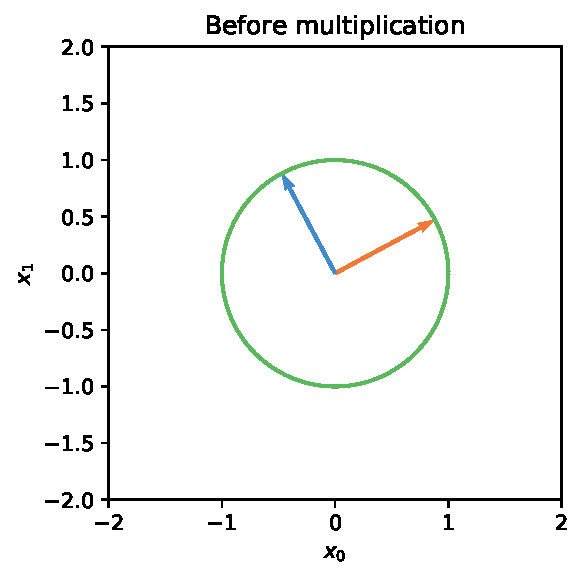
\includegraphics[width=0.48\textwidth]{../figures/week_1/unit_circle_before.pdf}
\hfill
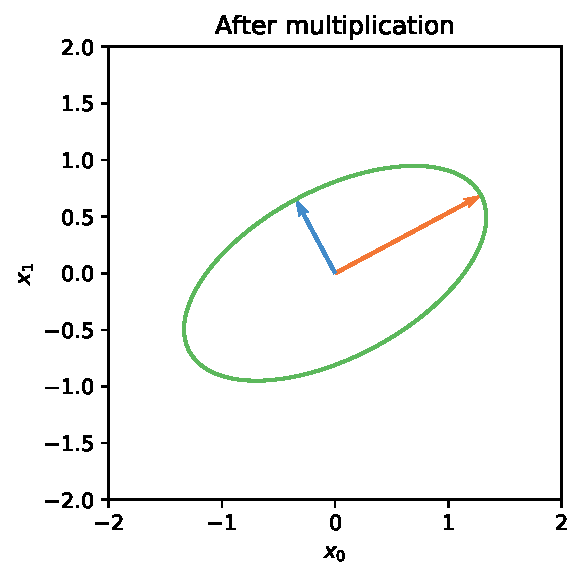
\includegraphics[width=0.48\textwidth]{../figures/week_1/unit_circle_after.pdf}
\end{center}

\end{frame}


\begin{frame}
\frametitle{Eigendecomposition}
    \begin{itemize}
        \item From the eigendecomposition we learn useful properties of the matrix.
        \item The eigendecomposition of a real symmetric matrix is used in optimization of quadratic expressions of the form $f(\vect{x}) = \vect{x}^T \vect{A} \vect{x}$ under the constraint $\norm{\vect{x}}_2 = 1$.
        \item For instance, if $\vect{x}=\vect{v}^{(i)}$, then $f(\vect{x}) = \lambda_i$, when $\vect{v}^{(i)}$ is an eigenvector of $A$ and $\lambda_i$ is its corresponding eigenvalue.
        \item The maximal (minimal) value of $f$ within the constraint region is equal to the maximal (minimal) eigenvalue.
    \end{itemize}

\end{frame}
\fi


\iffull
\begin{frame}
\frametitle{Trace}
    \begin{itemize}
        \item A {\bf trace} of a matrix is defined as
        $$Tr(\vect{A}) = \sum_{i} \vect{A}_{i,i} $$
        \item Expressions in terms of the trace operators allow to exploit many useful identities, e.g.
        $$Tr(\vect{A}\vect{B}\vect{C}) = Tr(\vect{B}\vect{C}\vect{A}) = Tr(\vect{C}\vect{A}\vect{B})$$
    \end{itemize}

\end{frame}
\fi

\fi % Linear algebra

\section{Gradient-based optimization}


\begin{frame}
\frametitle{Gradient-based optimization}
Materials:
\begin{itemize}
    \item Chapters I.4 and I.5 from \cite{deeplearning}
    \item \cite{linearalgebra}
\end{itemize}
\end{frame}

\begin{frame}
\frametitle{Gradient}
    \begin{itemize}
        \item Let $f: \R^{m \times n} \mapsto \R$ be a function that takes $m \times n$ matrix $\vect{A}$ as input and returns a real number (scalar).
        \item A {\bf gradient} of $f$ with respect to $A$ is the matrix
        $$
        \nabla_{\vect{A}} f(\vect{A}) =
        \begin{bmatrix}
         \frac{\partial f}{\partial A_{11}} & \frac{\partial f}{\partial A_{12}} & \ldots & \frac{\partial f}{\partial A_{1n}} \\
          \frac{\partial f}{\partial A_{21}} & \frac{\partial f}{\partial A_{22}} & \ldots & \frac{\partial f}{\partial A_{2n}} \\
          \vdots & \vdots & \ddots & \vdots \\
           \frac{\partial f}{\partial A_{m1}} & \frac{\partial f}{\partial A_{m2}} & \ldots & \frac{\partial f}{\partial A_{mn}}
        \end{bmatrix}
        $$
        \item i.e. an $m \times n$ matrix with  $$(\nabla_{\vect{A}} f(\vect{A}))_{ij} = \frac{\partial f}{\partial A_{ij}}  $$
        \item The size of the gradient of $\vect{A}$ is the same as the size of $A$.

    \end{itemize}
\end{frame}

\begin{frame}
\frametitle{Gradient}
    \begin{itemize}
        \item In the special case when $A$ is a vector we obtain the (possibly more familiar) gradient
        $$ \nabla_{\vect{x}} f(\vect{x}) =
        \begin{bmatrix}
         \frac{\partial f}{\partial x_{1}}  \\
          \frac{\partial f}{\partial x_{2}}  \\
          \vdots  \\
           \frac{\partial f}{\partial x_{m}}
        \end{bmatrix}$$
        \item In general to define a gradient we require that the function returns a {\bf real} value.
    \end{itemize}

\end{frame}

\begin{frame}
\frametitle{Jacobian}

\begin{itemize}
    \item The Jacobian $\vect{J_f}$ is a generalization of the gradient for vector valued functions.
    \item Let $\vect{f}:\R^n \mapsto \R^m $ be a function that takes $n$-dimensional vector $\vect{x}$ as input and returns a $m$-dimensional vector as an output.
    \item The Jacobian $\vect{J_f}$ is defined as
    $$
        \vect{J_f} =
        \begin{bmatrix}
         \frac{\partial f_1}{\partial x_{1}} & \frac{\partial f_1}{\partial x_{2}} & \ldots & \frac{\partial f_1}{\partial x_{n}} \\
          \frac{\partial f_2}{\partial x_{1}} & \frac{\partial f_2}{\partial x_{2}} & \ldots & \frac{\partial f_2}{\partial x_{n}} \\
          \vdots & \vdots & \ddots & \vdots \\
           \frac{\partial f_m}{\partial x_{1}} & \frac{\partial f_m}{\partial x_{2}} & \ldots & \frac{\partial f_m}{\partial x_{n}}
        \end{bmatrix}
    $$
    \item Note that for the special case of a scalar-valued function, the Jacobian is the transpose of the gradient.
\end{itemize}

\end{frame}

\begin{frame}
\frametitle{Optimization}

\begin{itemize}
    \item Most machine learning methods involve some kind of optimization.
    \begin{itemize}
        \item One exception is the $k$-Nearest neighbour classifier introduced later.
    \end{itemize}
    \item Optimization means minimizing or maximizing some function $f(\vect{x})$, i.e. finding the values of $\vect{x}$ for which $f(\vect{x})$ has a minimum or a maximum.
    \item Notation: $\vect{x}^* = \argmin f(\vect{x})$
\end{itemize}
\end{frame}


\begin{frame}{Gradient-based optimization}

\begin{itemize}
    \item The derivative tells us how to change $x$ in order to make a small improvement of $f(x)$.
    \item Therefore, derivatives can be useful in optimization.


\end{itemize}
\end{frame}


\section{Two simple machine learning models}


\begin{frame}
\frametitle{Two simple machine learning models}
Materials:
\begin{itemize}
    \item Chapter 2.3 from \cite{elements}
\end{itemize}

\end{frame}

\iffull
\begin{frame}
\frametitle{Some notations}
    \begin{itemize}
        \item We denote an input variable with the symbol $x$ (scalar) or $\vect{x}$ (vector).
        \item The $i$-th component of a vector input $\vect{x}$ is denoted as $x_i$.
        \item Quantitative (numerical) outputs are denoted with $y$.
        \item Qualitative outputs are denoted with $g$ (from group) and take values from a set $\cal{G}$.
        \item Matrices are denoted with bold and uppercase letters $\vect{X}$\\
        for instance, a set of $N$ input $p$-vectors $\vect{x}_i$ ($1 \leq i \leq N)$ is "packed" in a $N \times p$ input matrix $\vect{X}$.
        \item Since by default vectors are assumed to be column vectors, the rows of $\vect{X}$ are the transposes $\vect{x}_i^T$.
    \end{itemize}
\end{frame}
\fi

\begin{frame}
\frametitle{The learning task}
    \begin{itemize}
        \item Given a value of the input vector $\vect{x}$ make a good prediction of the output $y$, denoted as $\hat{y}$.
        \item Both $y$ and $\hat{y}$ should take values from the same numerical set.
        \item Similarly, $g$ and $\hat{g}$ should both take values from the same set $\cal{G}$.
         \item We suppose that we have available a set of measurements $(\vect{x}_i,y_i)$ or $(\vect{x}_i,g_i)$ $(1 \leq i \leq N)$ called {\bf training data} \\
         (in matrix form: $(\vect{X},\vect{y})$ and/or $(\vect{X},\vect{g})$).
        \item Our task is to construct a prediction rule based on the training data.

    \end{itemize}

\end{frame}


\begin{frame}
\frametitle{The learning task}
    Example:
    \begin{itemize}
         \item {\bf Variable values}: Let $g$ (and therefore also $\hat{g}$) be two valued (categorical), e.g. $\cal{G} = \{ \text{\textcolor{blue}{BLUE}, \textcolor{orange}{ORANGE}}\}$.
        \item {\bf Encoding of $g$s with $y$s}: Then each class can be encoded binary, i.e., with $y \in \{0,1\}$, e.g., \textcolor{blue}{BLUE} and \textcolor{orange}{ORANGE}, would correspond to $0$ and $1$, respectively.
        \item {\bf Predicted output values}: $\hat{y}$ ranges over the interval $[-\infty,+\infty]$ (of which $\{0,1\}$ is a subset).
        \item {\bf Prediction rule}: $\hat{g}$ is assigned a (class label) \textcolor{blue}{BLUE} if $\hat{y} < 0.5$ and \textcolor{orange}{ORANGE}, otherwise.

    \end{itemize}
\end{frame}



\begin{frame}
\frametitle{Two simple approaches to prediction}
\begin{itemize}
    \item Linear model fit
        \begin{itemize}
            \item strong assumptions about the structure of the decision boundary
            % \item stable but possibly inaccurate predictions
        \end{itemize}
    \item $k$-nearest neighbours
        \begin{itemize}
            \item weak assumptions about the structure of the decision boundary
            % \item predictions most often accurate but possibly unstable
        \end{itemize}
\end{itemize}

\end{frame}

\subsection{Linear model}

\begin{frame}
\frametitle{Linear model fit by least squares}
    \begin{itemize}
        \item Despite relative simplicity one of the most important statistical tools
        \item Input vector $\vect{x}^T = (x_1, x_2, \ldots, x_p)$
        \item Output $y$ predicted using the model \\
            \begin{center}
            $\hat{y} = \hat{w_0} + \sum_{j=1}^{p} x_j \hat{w_j}$
            \end{center}
        \item $\hat{w}_i$ $ (0 \leq i \leq p)$ are the parameters of the linear model
        \item In vector form
            \begin{center}
            $\hat{y} = \hat{\vect{w}}^T\vect{x} = \vect{x}^T \hat{\vect{w}}$
            \end{center}
            using the fact that the scalar (inner) product of two vectors is a commutative operation.
    \end{itemize}
\end{frame}

\begin{frame}
\frametitle{Linear model fit by least squares}
    \begin{itemize}
        \item  We assume that $w_0$ is in $\vect{w}$ and $1$ is included in $\vect{x}$.
        \item $\hat{y}$ is a scalar, but in general can be a $k$-vector $\hat{\vect{y}}$, in which case $\vect{w}$ becomes a $p \times k$ matrix of coefficients.
    \end{itemize}
\end{frame}

\iffull
\begin{frame}
\frametitle{Linear model fit by least squares}
    Some hyper(space) terminology:
    \begin{itemize}
        \item Points $\vect{x},\hat{y}$ form a {\bf hyperplane} in the $(p+1)$-dimensional input-output hyperspace.
        \item If $\vect{x}$ is extended with constant $1$ then the hyperplane includes the origin and it forms a {\bf subspace}.
        \item If $1$ is not included then the hyperplane is an {\bf affine} set and it cuts the $y$-axis at the point $(\vect{0}, \hat{w_0})$, where the vector $\vect{0}$ has all $x_i$ coordinates equal to $0$.
        \item Reminder: from now on we assume that $1$ is included in $\vect{x}$ and $\hat{w_0}$ in $\hat{\vect{w}}$/
        \item The function $f(\vect{x}) =  \vect{w}^T \vect{x}$ defined on the $p$-dimensional (input) space is a {\bf linear} function (we omit the hats over the $w$s since now we consider them as free variables).
        \item The gradient $\nabla f(\vect{x})$ is a vector pointing along the direction of maximal change.
    \end{itemize}
\end{frame}
\fi

\begin{frame}
\frametitle{Linear model fit by least squares}
\frametitle{}
    \begin{itemize}
        \item There are many ways to fit a linear model to a training dataset.
        \item {\bf Least squares} method
            \begin{itemize}
                \item We need to find coefficients $\hat{w_i}$ which minimize the error estimated with the {\bf residual sum of squares}
                \begin{center}
                    $$\mbox{RSS}(\vect{w}) = \sum_{i = 1}^{N}(y_i - \vect{x}_i^T \vect{w})^2$$
                \end{center}
                 assuming $N$ input-output pairs.
            \end{itemize}
        \item $\mbox{RSS}(\vect{w})$ is a quadratic function.
        \item A minimum always exists though not necessarily a unique one.
    \end{itemize}

\end{frame}


\begin{frame}
\frametitle{Linear model fit by least squares}
    \begin{itemize}
        \item We look for the solution $\hat{\vect{w}}$ using the matrix notation:
        \item $\vect{y} = [y_1, y_2, \ldots, y_N]^T$ is the vector formed from the $N$ output vectors and $\vect{X}$ is an $N \times p$ matrix  \\
        % (\vect{y} - \vect{X}^T \vect{w})^2 =
        $$\mbox{RSS}(\vect{w}) =  (\vect{y} - \vect{X} \vect{w})^T (\vect{y} - \vect{X} \vect{w})$$
        \item To find the minimum we differentiate with respect to $\vect{w}$ which gives
        %$$(-\vect{X})^T(\vect{y}-\vect{X}\vect{w}) + (\vect{y}-\vect{X}\vect{w})^T (-\vect{X})$$
        %using the rule $(\vect{A}\vect{B})^T = \vect{B}^T\vect{A}^T$ this is equivalent to
        $$ -2 \vect{X}^T(\vect{y}-\vect{X}\vect{w})$$
    \end{itemize}
    
\vfill
\tiny{For details about the derivation check equations 4 and 5 in \href{https://web.stanford.edu/~mrosenfe/soc_meth_proj3/matrix_OLS_NYU_notes.pdf}{this document}.}

\end{frame}

\begin{frame}
\frametitle{Linear model fit by least squares}
    \begin{itemize}

    \item To find the minimum our derivative must be $\vect{0}$, hence:
        $$\vect{X}^T(\vect{y}-\vect{X}\vect{w}) =  \vect{0}$$
        $$\vect{X}^T \vect{y} -\vect{X}^T\vect{X}\vect{w} =  \vect{0}$$
        $$ \vect{X}^T \vect{y} = \vect{X}^T\vect{X}\vect{w}$$
    \item    If $\vect{X}^T\vect{X}$ is non-singular there exists a unique solution given by
        $$\hat{\vect{w}} = (\vect{X}^T\vect{X})^{-1}\vect{X}^T \vect{y}$$
    \end{itemize}

\end{frame}

\iffull
\begin{frame}
\frametitle{Discussion point 1}

Why we cannot simply solve for $\hat{\vect{w}}$ in the following way?

$$\vect{y} -\vect{X}\vect{w}=  \vect{0}$$ 
$$\vect{y} = \vect{X}\vect{w}$$ 
$$\hat{\vect{w}} = \vect{X}^{-1} \vect{y}$$

\end{frame}
\fi

\begin{frame}{Linear model fit by least squares}
    \begin{itemize}
        \item For each input $\vect{x}_i$ there corresponds the fitted output $$\hat{y}_i = \hat{y}_i(\vect{x}_i) = \hat{\vect{w}}^T\vect{x}_i$$.
        \item This is called ``making a prediction'' for $\vect{x}_i$.

        \item The entire fitted surface (hyperplane) is fully characterized by the parameter vector $\hat{\vect{w}}$.

        \item After fitting the model, we can ``discard'' the training dataset.
    \end{itemize}
\end{frame}

\begin{frame}
\frametitle{Example: Linear model fit by least squares}
\begin{itemize}
    \item Scatter plot (on next slide) of training data on a pair of inputs $x_1$ and $x_2$
    \item Output class variable $g$ has two values \textcolor{blue}{BLUE} and \textcolor{orange}{ORANGE}.
    \item Linear regression model fitted with the response variable $y$ coded as $0$ for \textcolor{blue}{BLUE} and $1$ for \textcolor{orange}{ORANGE}.
    \item Fitted values $\hat{y}$ converted to a fitted class variable $\hat{g}$ as
    \[ \hat{g} = \begin{cases}
                    \text{\textcolor{blue}{BLUE}}  & \text{if $\hat{y} \leq 0.5$} \\
                    \text{\textcolor{orange}{ORANGE}} & \text{if $\hat{y} > 0.5$ }
                 \end{cases} \]

\end{itemize}
\end{frame}

\begin{frame}{Example: Linear model fit by least squares}
    \begin{center}
        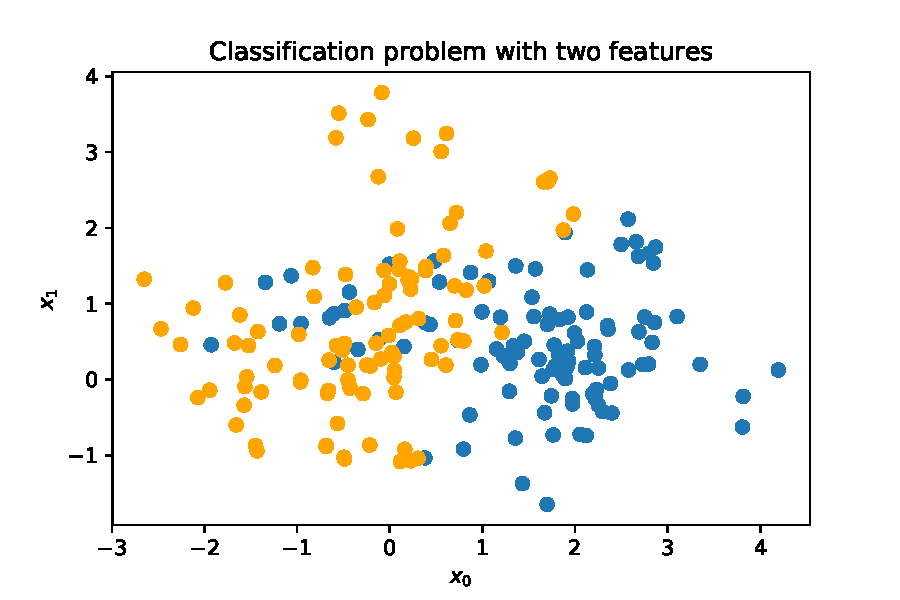
\includegraphics[width=0.48\textwidth]{../figures/week_1/classification_problem.pdf}
        \hfill
        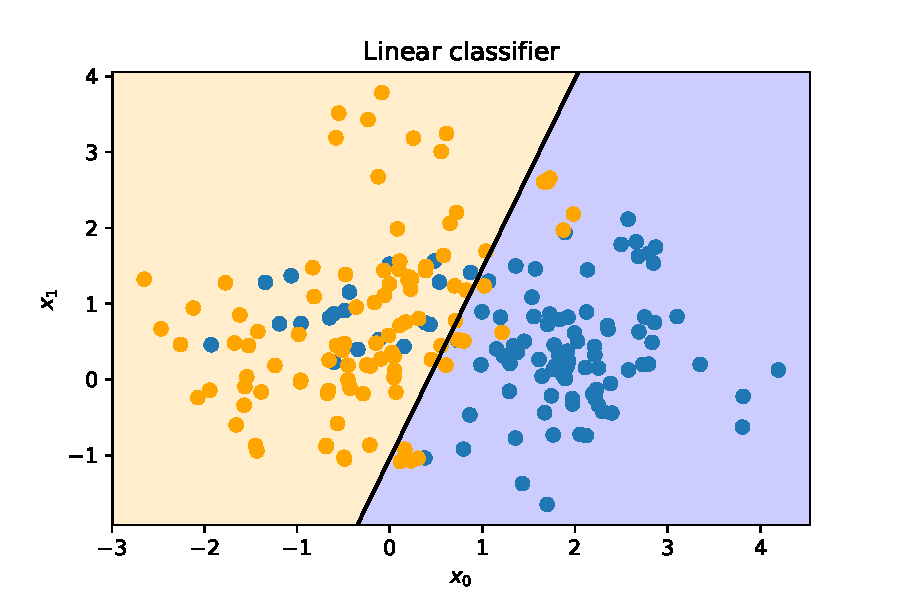
\includegraphics[width=0.48\textwidth]{../figures/week_1/linear_model.pdf}
        \end{center}
\end{frame}

\iffull
\begin{frame}
\frametitle{Example: Linear model fit by least squares}
\begin{itemize}
    \item Two classes separated in the plane ($\R^2$) by the decision boundary $\{ \vect{x} : \vect{w}^T\vect{x} = 0.5 \}$
    \item $\{ \vect{x} : \vect{w}^T\vect{x} < 0.5 \}$ set of \textcolor{blue}{BLUE} points
    \item $\{ \vect{x} : \vect{w}^T\vect{x} \geq 0.5 \}$ set of \textcolor{orange}{ORANGE} points

\end{itemize}
\end{frame}
\fi

\begin{frame}
\frametitle{Example: Linear model fit by least squares}
\begin{itemize}
    \item Wrong classifications on both sides of the boundary
    \item Are the errors caused by the model or are they unavoidable?
    \item Two possible scenarios
        \begin{itemize}
            \item {\bf Scenario 1}: data generated from bivariate Gaussian distribution
            \item {\bf Scenario 2}: data generated from 10 Gaussian distributions; the means of these distributions are also distributed as Gaussian
        \end{itemize}
    \item In Scenario 1 the linear boundary is the best we can do since the overlap is inevitable.
    \item In Scenario 2 the linear boundary is unlikely to be optimal \\
          (in fact the boundary is non-linear and disjoint).
\end{itemize}

\end{frame}


\subsection{Nearest-neighbours model}

\begin{frame}
\frametitle{Nearest-neighbours model}
    \begin{itemize}
        \item In nearest-neignbour methods $\hat{y}(\vect{x})$ is determined based on the inputs (points) in the training set $\cal{T}$ which are "closest" to the input $\vect{x}$.
        \item $k$-nearest neighbour fit is defined as
        $$ \hat{y}(\vect{x}) = \frac{1}{k} \sum_{\vect{x}_i \in N_k(\vect{x})} y_i $$
        where $N_k(\vect{x})$ is the neighbourhood of $\vect{x}$ consisting of the $k$ "closest" points to $\vect{x}$.
        \item "Closeness" requires a definition of {\bf metrics}.
        \item For the moment we assume Euclidian distance (each $\vect{x}$ is a point in the hyperspace).
        \item An average of the classes of the $k$ closest points (but only for binary classification problem.
    \end{itemize}
\end{frame}

\begin{frame}
\frametitle{Back to the \textcolor{blue}{BLUE} and \textcolor{orange}{ORANGE} example}
    \begin{itemize}
        \item We use the same training data as in the linear model example.
        \item New borderline between the classes generated with 15-nearest-neighbour model.
        \item Since \textcolor{orange}{ORANGE} is encoded as 1 $\hat{y}$ is the proportion of \textcolor{orange}{ORANGE} points in the 15-neighbourhood.
        \item Class \textcolor{orange}{ORANGE} assigned to $\vect{x}$ if $\hat{y}(\vect{x}) > 0.5$ (majority is \textcolor{orange}{ORANGE}).
    \end{itemize}
\end{frame}

\begin{frame}
\frametitle{15-Nearest neighbour classifier}
    \begin{center}
        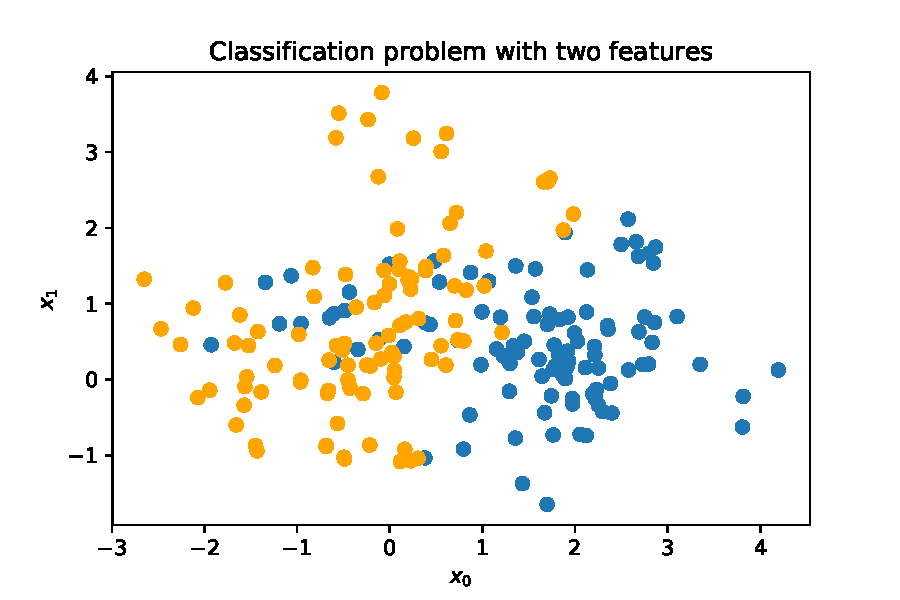
\includegraphics[width=0.48\textwidth]{../figures/week_1/classification_problem.pdf}
        \hfill
        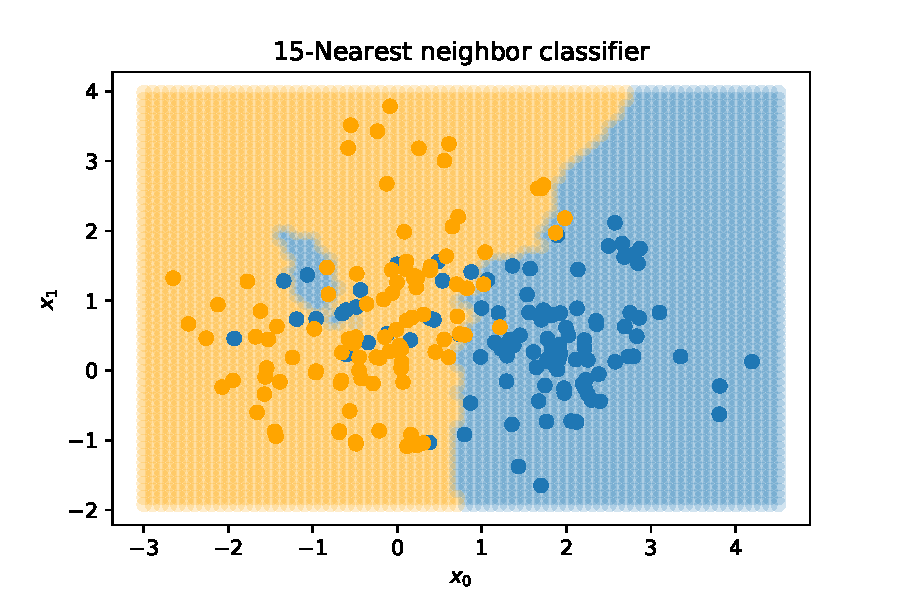
\includegraphics[width=0.48\textwidth]{../figures/week_1/15-nn.pdf}
    \end{center}
\end{frame}

\begin{frame}
\frametitle{Linear classifier vs. 15-Nearest neighbour}
    \begin{center}
        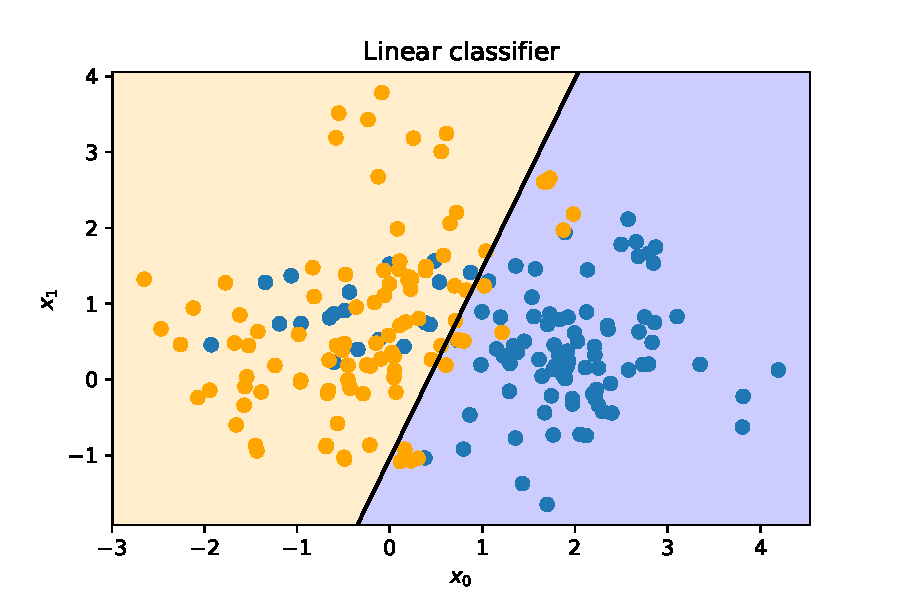
\includegraphics[width=0.48\textwidth]{../figures/week_1/linear_model.pdf}
        \hfill
        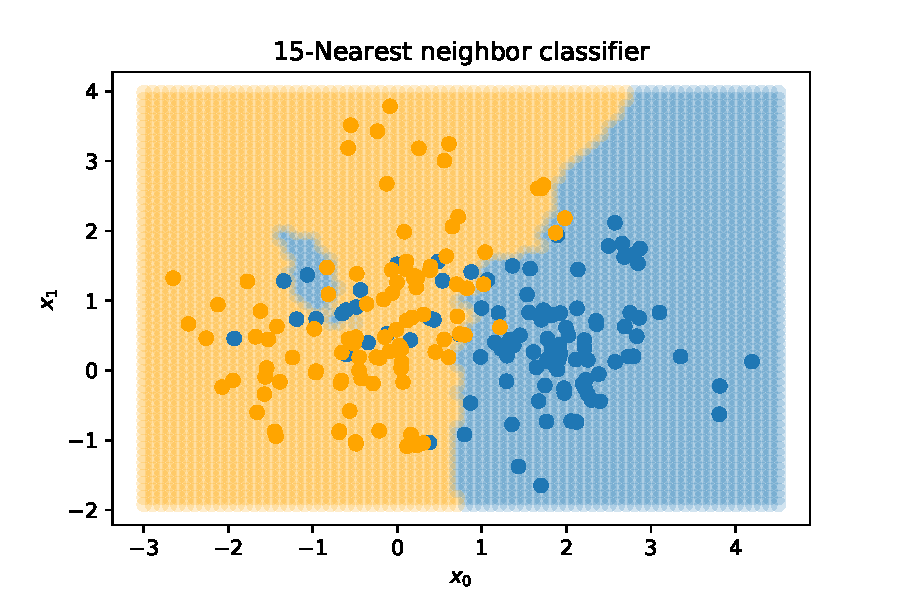
\includegraphics[width=0.48\textwidth]{../figures/week_1/15-nn.pdf}
    \end{center}
\end{frame}


\begin{frame}
\frametitle{1-Nearest neighbour vs. 15-Nearest neighbour}
    \begin{center}
        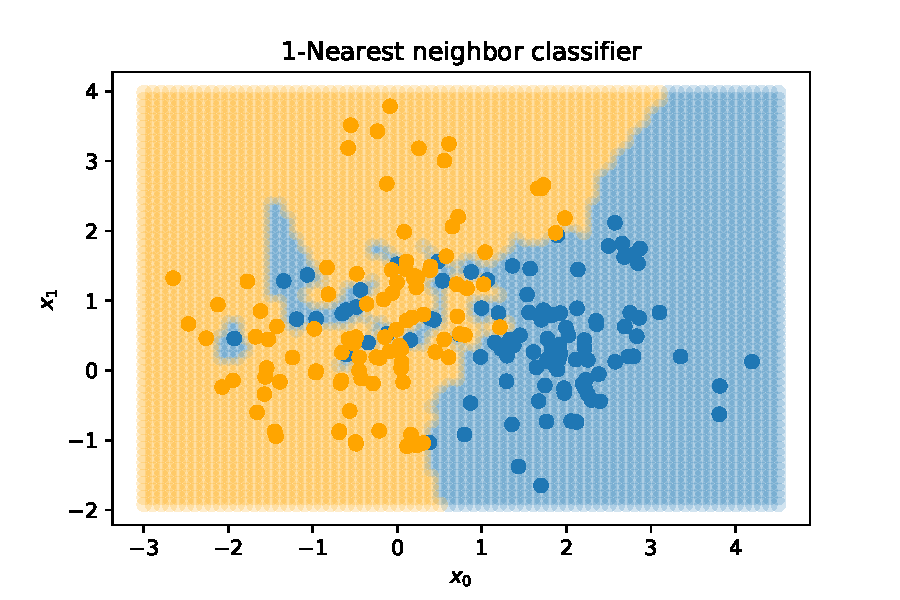
\includegraphics[width=0.48\textwidth]{../figures/week_1/1-nn.pdf}
        \hfill
        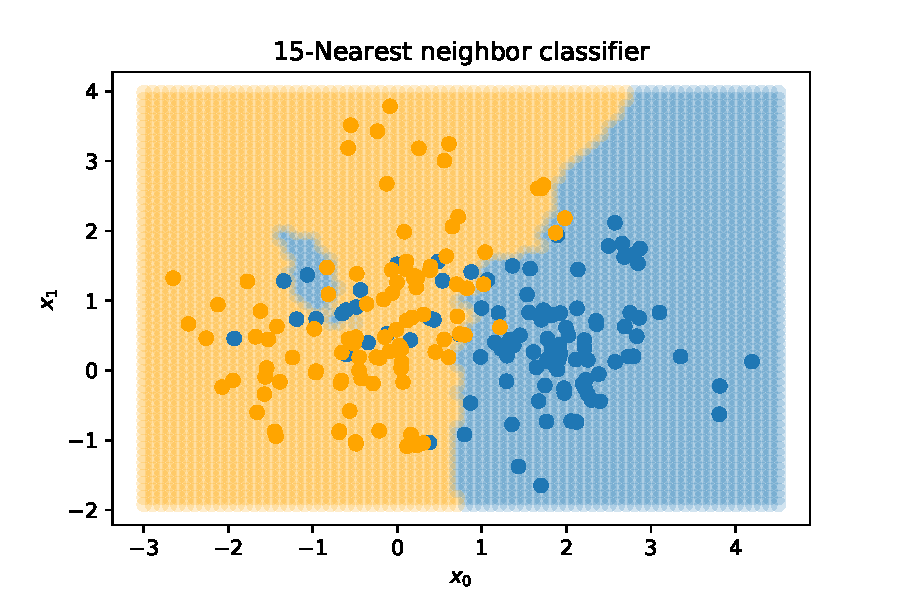
\includegraphics[width=0.48\textwidth]{../figures/week_1/15-nn.pdf}
    \end{center}
\end{frame}

\iffull
\begin{frame}
\frametitle{Comparison of the techniques}
    \begin{itemize}
        \item 15-NN seems to work better than the linear classifier since fewer points are missclassified.
        \item On the other hand, {\bf none} of the points in the 1-NN case was misclassified!?
        \item Actually with the 1-NN method the error on {\bf training data} is always 0.
        \item An independent test set needed to obtain a better comparison of the methods.
    \end{itemize}
\end{frame}
\fi


\begin{frame}
\frametitle{Comparison of techniques}

    \begin{itemize}
        \item At first sight it looks like k-NN has only one parameter, $k$ versus $p$ parameters (number of weights $w_i$) of the linear model.
        \item The {\bf effective}  number of parameters of k-NN is $N/k$ which is in general bigger than $p$ ($N$ is the size of the training set).
        \item For instance, assume non-overlapping neighbourhoods
            \begin{itemize}
                \item There will be $N/k$ neighbourhoods.
                \item To each neighbourhood there correspond one parameter (the mean of the elements of the neighbourhood).
            \end{itemize}
    \end{itemize}

\end{frame}

\iffull
\begin{frame}
\frametitle{Discussion point 2}
Assume that you are building a machine learning model to be used as an \textit{aid} by clinicians for decision making. The inputs to the model are a number of \textit{biomarkers} describing the condition of the patient.
\\~\

The clinician specifies that they are interested in a model that is \textit{interpretable}, i.e. a model that will not only output a prediction but also give an indication about which biomarkers are important when making the prediction.
\\~\

You can either use a linear model or a $k$-NN classifier. What is the better choice in your opinion?

\end{frame}
\fi

\iffull % Probability theory
\section{Probability theory}

\begin{frame}
\frametitle{Probability theory}

Materials:
\begin{itemize}
    \item Chapter I.3 from \cite{deeplearning}
\end{itemize}
\end{frame}

\begin{frame}
\frametitle{Probability theory}
\begin{itemize}
    \item Probability theory is a mathematical framework for dealing with uncertainty, i.e., modeling and analyzing uncertain events and statements
    \item In AI probability theory is used in two major ways:
        \begin{itemize}
            \item To design AI systems, i.e., derive models and expressions and the corresponding algorithms.
            \item To analyze the behaviour of the AI systems.
        \end{itemize}

\end{itemize}

\end{frame}

\begin{frame}
\frametitle{Probability theory}
    \begin{itemize}
        \item A {\bf random variable} is a variable that can take values randomly.
        \iffull
        \item We will denote random variables with plain (ordinary text) typeface and their values with standard math typeface\\
        for example, if the random variable is denoted as x its values can be $x_1$ and $x_2$.
        \item A vector-valued random variable is denoted with bold typeface, e.g. {\bf x}.
        \fi
        \item On its own a random variable just denotes the set of its possible values; to get its full meaning in needs to be coupled with a distribution.
    \end{itemize}
\end{frame}


\begin{frame}
\frametitle{Probability theory}
    \begin{itemize}
        \item There are two types of random variables: {\bf discrete} and {\bf continuous}.
        \item Consequently there are two ways to describe probability distributions: {\bf probability mass functions} and {\bf probability density functions}.
    \end{itemize}
\end{frame}


\begin{frame}
\frametitle{Probability mass function}
\begin{itemize}
    \item The domain of a probability mass function $P$ is the set of all possible states of the random variable x.
    \item $\forall x \in \text{x}: 0 \leq P(\text(x) \leq 1$
        \begin{itemize}
            \item An impossible event has probability 0 and no state can be less probable than that.
            \item An event that is guaranteed to happen has probability 1 and no state can have a greater chance of occurring.
        \end{itemize}
    \item $\sum_{x \in \text{x}} P(x) = 1$
        \begin{itemize}
            \item We say that \text{x} is {\bf normalized}.
        \end{itemize}
    \item Example: Uniform distribution: $P(\text{x} = x_i) = \frac{1}{k}$.
\end{itemize}
\end{frame}


\begin{frame}
\frametitle{Probability density function}
\begin{itemize}
    \item The domain of the probability density function $p$ must be the set of all possible states of $\text{x}$.
    \item $\forall x \in \text{x}: p(x)\geq 0.$
    \item $$\int p(x)dx = 1$$
    \item Example: uniform distribution $u(x;a,b) = \frac{1}{b-a}$, for $x \in [a,b]$
\end{itemize}

\end{frame}


\begin{frame}
\frametitle{Conditional probability}
    \begin{itemize}
        \item {\bf Conditional probability} is the probability of some event provided that some other event has happened.
        \item
        Given two random variables x and y, the conditional probability that y has value $y$ provided that we know that x has value $x$ is given by
        $$
        P(\text{y}=y \mid \text{x} = x) = \frac{P(\text{x,y})}{P(\text{x}=x)}
        $$
        \item Another way to see this formula is $$P(\text{x,y}) = P(\text{x} = x)P(\text{y} = y \mid \text{x} = x)$$ i.e., the probability of $x$ and $y$ occurring together is equal to the probability of occurrence of $x$ times the probability of $y$ occurring provided $x$ has occurred.
    \end{itemize}

\end{frame}





\begin{frame}
\frametitle{Expectation}
\begin{itemize}
    \item The {\bf expectation} or {\bf expected} value of a function $f(x)$ with respect to a probability distribution $P(x)$ is the average value of $f$ over all values $x$ assuming they are drawn from $P$
    \item $$\field{E}_{\text{x} \sim P} [f(x)] = \sum_{x} P(x) f(x)$$
    \item $$\field{E}_{\text{x} \sim P} [f(x)] = \int p(x) f(x) dx$$
    \item Linarity of expectations:
    $$\field{E}_{\text{x}} [\alpha f(x) + \beta g(x)] =  \alpha \field{E}_\text{x}[f(x)] + \beta \field{E}_\text{x}[g(x)]$$
\end{itemize}

\end{frame}



\begin{frame}
\frametitle{Variance and covariance}
\begin{itemize}
    \item The {\bf variance} gives a measure of variation of the values of a random variable x $$\mbox{Var}(f(x)) = \field{E}[(f(x) - E[f(x)])^2]$$
    Square root of the variance is called {\bf standard deviation}.

    \item The {\bf covariance} is a measure of linear relation as well as scale between $$\mbox{Cov}(f(x),g(x)) = \field{E}[f(x) - E[(f(x)])(g(x) - E[g(x)])]$$
\end{itemize}

\end{frame}


\begin{frame}
\frametitle{Covariance matrix}
    \begin{itemize}
        \item The {\bf covariance matrix} of a random vector $\vect{x} \in \R^n$ is a $n \times n$ matrix with elements
    $$
    \mbox{Cov}(\vect{x})_{i,j} = \mbox{Cov}(x_i,x_j)
    $$
    \item The diagonal elements of the matrix give the variance
    $$
      \mbox{Cov}(\text{x}_i,\text{x}_i) = \mbox{Var}(\text{x}_i)
    $$
    \end{itemize}

\end{frame}



\begin{frame}
\frametitle{Bernouli Distribution}
\begin{itemize}
    \item A distribution over a single binary random variable
    \item Controlled by a single parameter $\phi \in [0,1]$ which corresponds to the probability of the random variable taking the value 1
    \item Properties:
    \begin{eqnarray*}
    P({\rm x}) = 1) = \phi \\
    P({\rm x} = 0) = 1 - \phi \\
    P({\rm x} = x) = \phi^x (1-\phi)^{1-x} \\
    \field{E}_\text{x}[\text{x}] = \phi \\
    Var(\text{x}) = \phi(1-\phi)
    \end{eqnarray*}
\end{itemize}
\end{frame}

\begin{frame}
\frametitle{Gaussian distribution}
\begin{itemize}
    \item The most commonly used distribution, also called {\bf normal distribution}.
    \item Controlled by two parameters $\mu \in \R$ (the {\bf mean}) and $\sigma \in (0, \infty)$, (the {\bf standard deviation})

    $$
    {\cal N}(x ; \mu, \sigma^2) = \sqrt{\frac{1}{2 \pi \sigma^2}} \mbox{exp} \left (-\frac{1}{2 \sigma^2}(x - \mu)^2 \right )
    $$

    $$
    {\cal N}(\vect{x} ; \vect{\mu}, \vect{\Sigma}) = \sqrt{\frac{1}{(2 \pi)^n \mbox{det}(\Sigma)}} \mbox{exp} \left (-\frac{1}{2} (\vect{x} - \vect{\mu})^T \vect{\Sigma}^{-1} (\vect{x} - \vect{\mu}) \right )
    $$


\end{itemize}
\end{frame}


\begin{frame}
\frametitle{Gaussian distribution}
\begin{center}
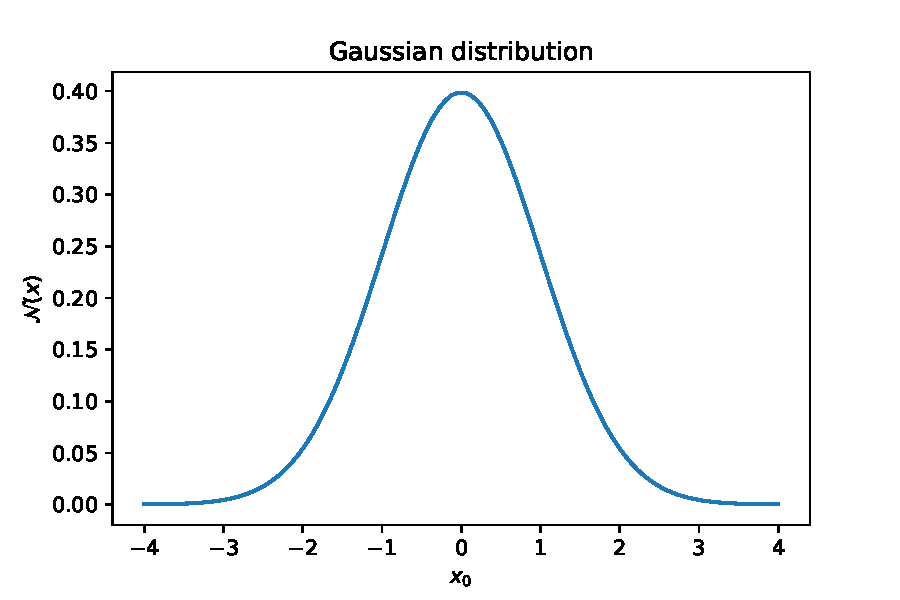
\includegraphics[width=0.48\textwidth]{../figures/week_1/gaussian_1d.pdf}
\hfill
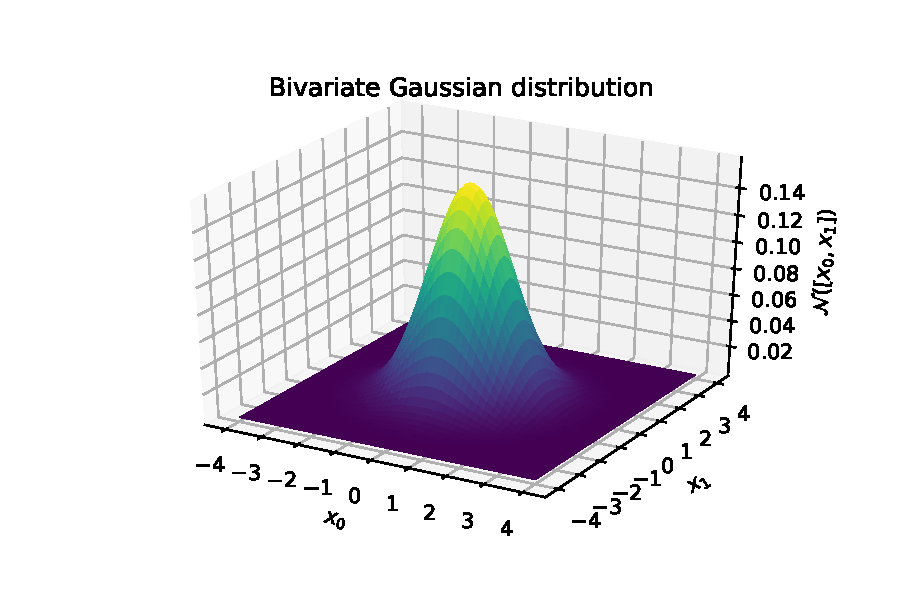
\includegraphics[width=0.48\textwidth]{../figures/week_1/gaussian_2d.pdf}
\end{center}
\end{frame}

\begin{frame}
\frametitle{Logistic sigmoid}
\begin{itemize}
    \item A useful function that we are going to consider
    $$\sigma(x) = \frac{1}{1 + \exp{(-x)}}$$
    \item The Logistic (sigmoid) function is commonly used to parametrize Bernoulli distributions.
    \begin{center}
    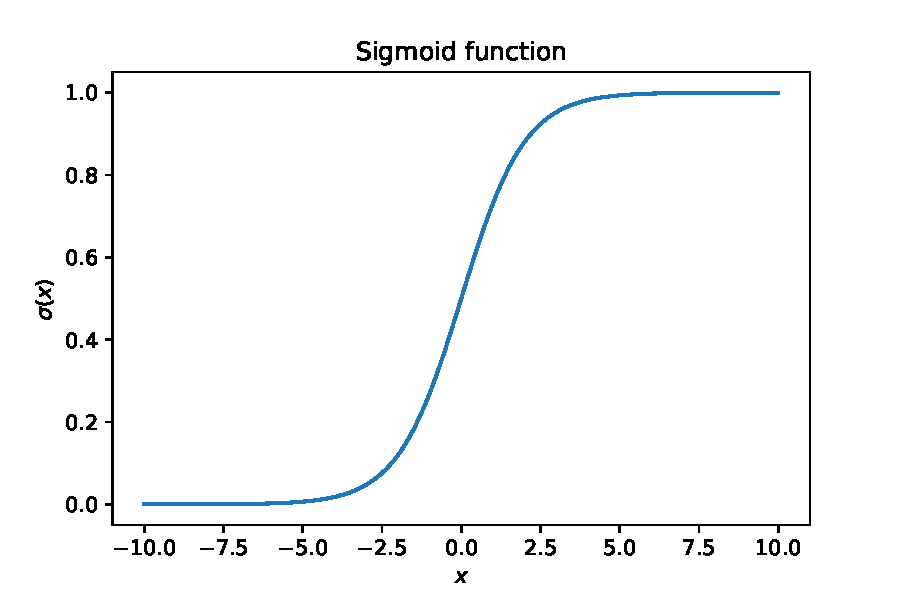
\includegraphics[width=0.48\textwidth]{../figures/week_1/sigmoid.pdf}
    \end{center}

\end{itemize}
\end{frame}


\begin{frame}
\frametitle{Bayes' rule}
\begin{itemize}
    \item Suppose know $P(\text{y} \mid \text{x})$, but we actually need $P(\text{x} \mid \text{y})$. If we know $P(\text{x})$ then we can compute
    $$
        P(\text{x} \mid \text{y}) = \frac{P(\text{y} \mid \text{x})P(\text{x})}{P(\text{y})}
    $$
    Although it appears in the formula prior knowledge $P(\text{y}$ is not needed since usually it can be computed as $\sum_{\text{x}} P(\text{y} \mid \text{x})P(\text{x})$
    \item It can be straightforwardly derived from the conditional probability formula.
    \item It could have be named also after Laplace who independently found it, generalized it, and introduced it in practice.
\end{itemize}
\end{frame}

\fi % Probability theory


\section{Model capacity, underfitting and overfitting}

\begin{frame}
\frametitle{Model capacity, underfitting and overfitting}
Materials:
\begin{itemize}
    \item Chapter I.5.2 from \cite{deeplearning}
\end{itemize}
\end{frame}

\begin{frame}
\frametitle{Linear regression}
    \begin{center}
            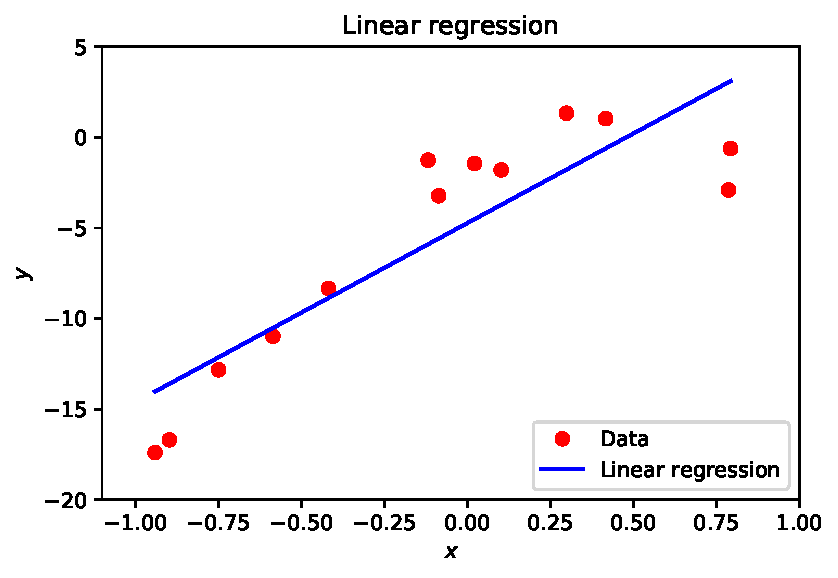
\includegraphics[width=0.75\textwidth]{../figures/week_1/linear_regression.pdf} \\
            $\hat{y} = \hat{w_0} + \sum_{i=1}^{n} x_i \hat{w_i}$ \\
            $\hat{y} = \vect{x}^T \hat{\vect{w}}$
    \end{center}
\end{frame}

\begin{frame}
\frametitle{Generalization}
    \begin{itemize}
        \item The central challenge in machine learning is to design an algorithm which will perform well on new data (different from the training set data).
        \item This ability is called {\bf generalization}.
        \item {\bf Training error} is the error computed on the training set.
        \iffull
        \item During the training (learning) we aim at reducing the training error.
        \item If that is the end goal, we only have an optimization problem, not a machine learning one.
        \fi
    \end{itemize}
    \begin{center}
            \iffull
            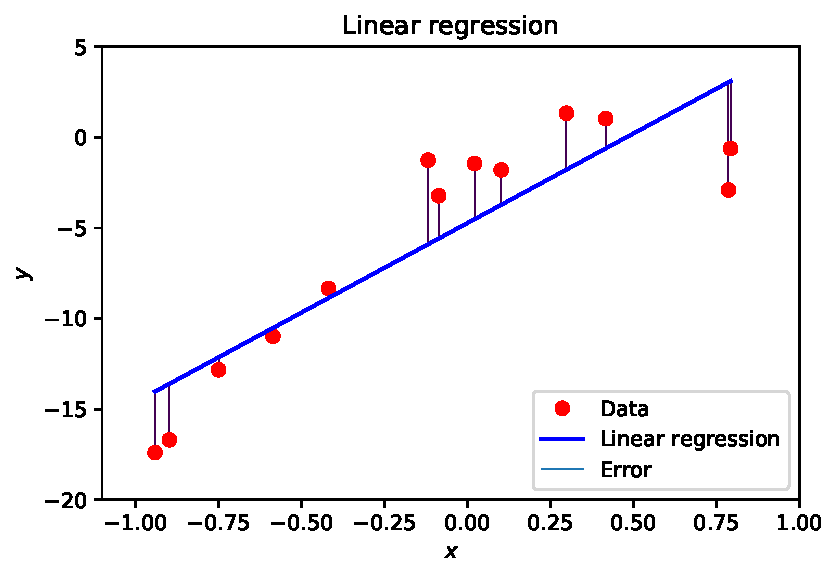
\includegraphics[width=0.3\textwidth]{../figures/week_1/linear_regression_error.pdf}
            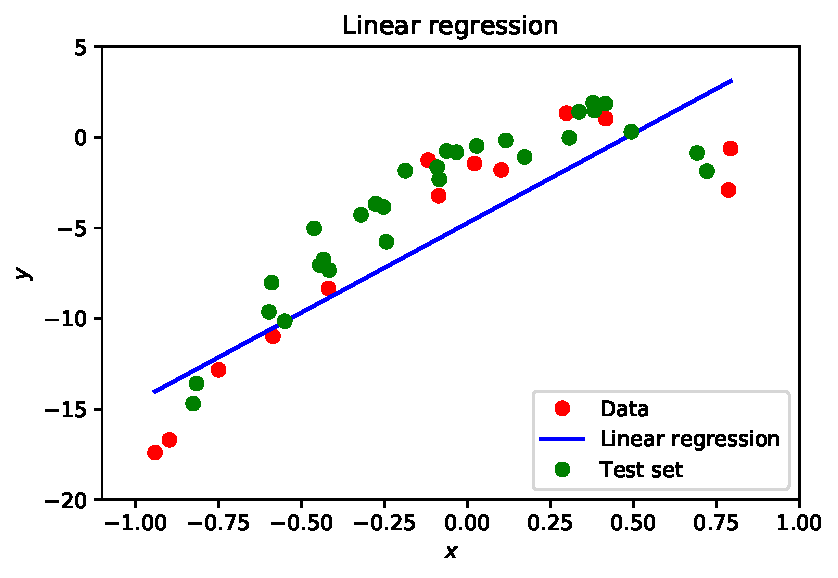
\includegraphics[width=0.3\textwidth]{../figures/week_1/linear_regression_test_set.pdf}
            \else
            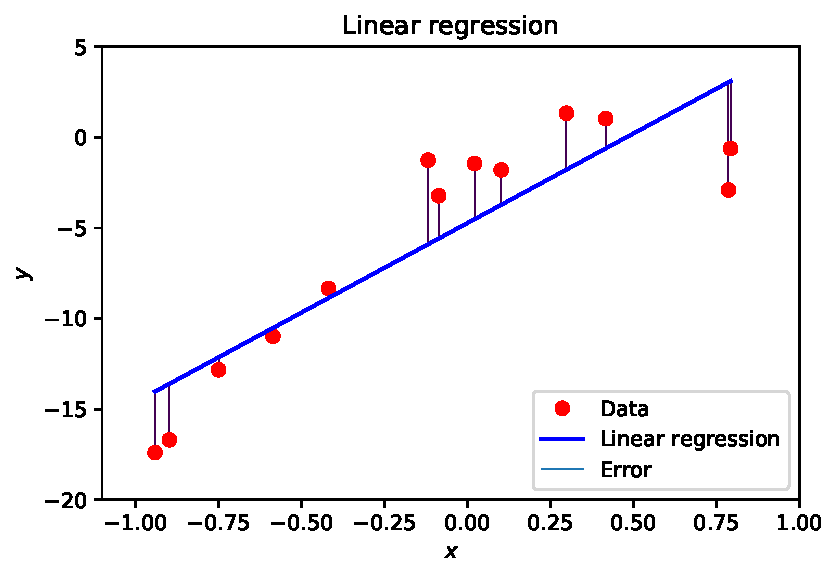
\includegraphics[width=0.47\textwidth]{../figures/week_1/linear_regression_error.pdf}
            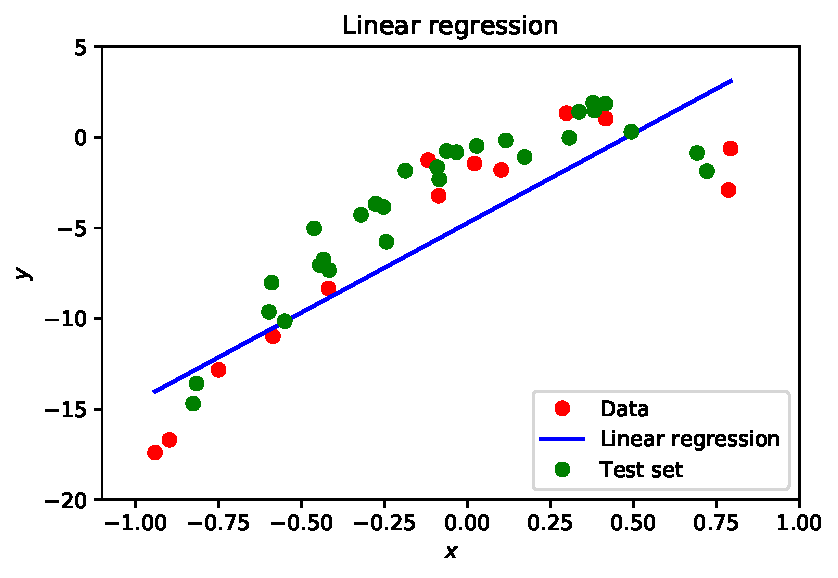
\includegraphics[width=0.47\textwidth]{../figures/week_1/linear_regression_test_set.pdf}
            \fi
    \end{center}
\end{frame}

\iffull
\begin{frame}
\frametitle{Generalization error}
    \begin{itemize}
        \item {\bf Generalization error}, also called {\bf test error} is defined as the expected error on new, previously unseen data.
        \item Unlike in simple optimization, in machine learning our main goal is to minimize the {\bf generalization error}.
        \item Usually the generalization error is estimated by measuring the performance on a {\bf test data set} which must be independent from the training set.
    \end{itemize}
\end{frame}
\fi

\begin{frame}
\frametitle{Example: Linear regression}
 \begin{itemize}
        \item Previously, we trained the model by minimizing the training error
        $$
        \frac{1}{m^{\mbox{(train)}}}\norm{\vect{X}^{\mbox{(train)}}\hat{\vect{w}} - \vect{y}^{\mbox{(train)}}}_2^2
        $$
        \item We would like actually to minimize the test error
         $$
        \frac{1}{m^{\mbox{(test)}}}\norm{\vect{X}^{\mbox{(test)}}\hat{\vect{w}} - \vect{y}^{\mbox{(test)}}}_2^2
        $$
\end{itemize}
\begin{center}
        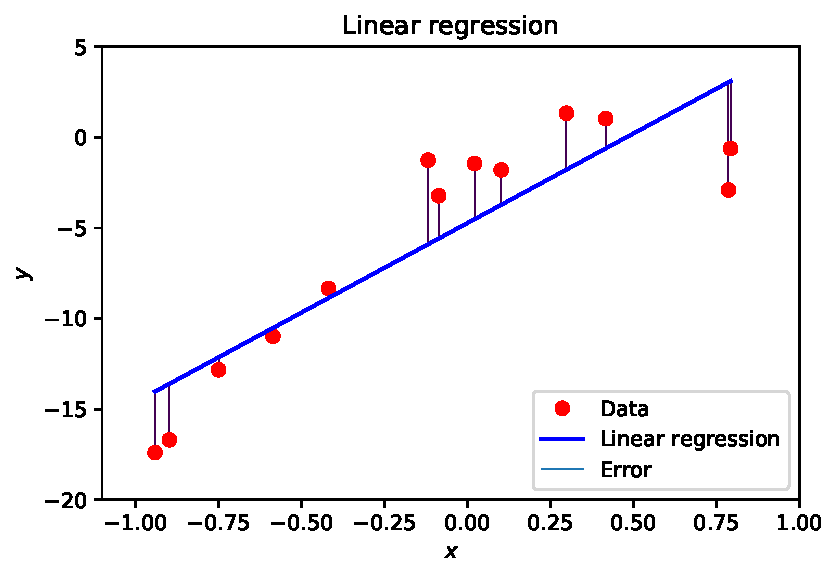
\includegraphics[width=0.47\textwidth]{../figures/week_1/linear_regression_error.pdf}
        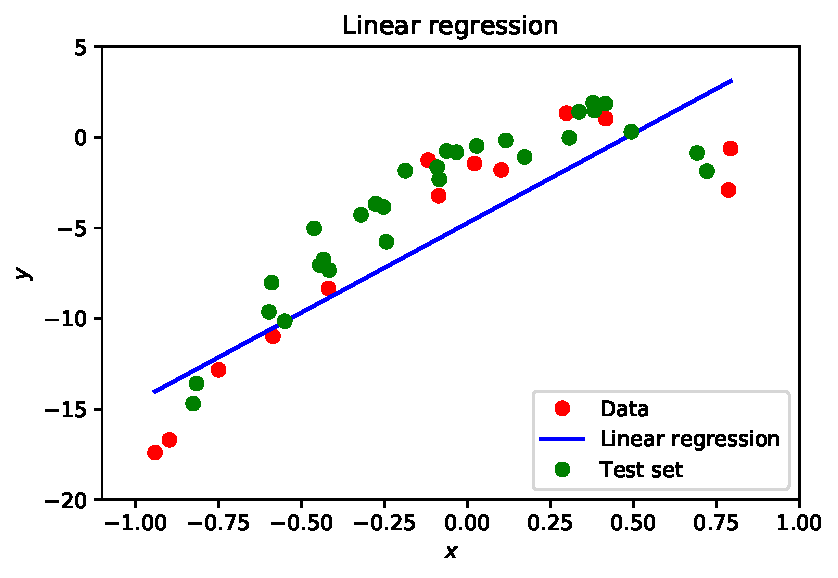
\includegraphics[width=0.47\textwidth]{../figures/week_1/linear_regression_test_set.pdf}
\end{center}
\end{frame}


\begin{frame}
\frametitle{Statistical learning theory}
    \begin{itemize}
        \item {\bf Statistical learning theory} provides methods to mathematically reason about the performance on the test set although we can observe only the training set.
        \item This is possible under some assumptions about the data sets
            \begin{itemize}
                \item The training and test data are generated by drawing from a probability distribution over data sets. We refer to that as {\bf data-generating process}.
                \item {\bf i.i.d. assumptions}
                    \begin{itemize}
                        \item Examples in each data sets are {\bf independent} from each other.
                        \item The training data set and the test data set are {\bf identically distributed}, i.e., drawn from the same probability distribution.
                    \end{itemize}
            \end{itemize}

    \end{itemize}
\end{frame}

\iffull
\begin{frame}
\frametitle{Discussion point 3}
Can you name a scenario in medical image analysis practice where the i.i.d. assumptions are bound to be broken?
\end{frame}


\begin{frame}
\frametitle{Underfitting and overfitting}
    \begin{itemize}
        \item The factor that determines how well a machine algorithm will perform is its ability to
            \begin{enumerate}
                \item Make the training error small.
                \item Make the difference between the training and test error small.
            \end{enumerate}
        \item These two factors correspond to the two central challenges in machine learning: {\bf underfitting} and {\bf overfitting}.
        \iffull
        \item Underfitting occurs when the model is not able to produce a sufficiently small training error.
        \item Overfitting occurs when the gap between the training and test errors is too large.
        \fi
    \end{itemize}
\end{frame}
\fi

\begin{frame}
\frametitle{Model capacity}
    \begin{itemize}
        \item A {\bf capacity of the model} is its ability to fit a wide variety of functions.
        \iffull
        \item Low capacity models struggle to fit the training set (underfitting).
        \item Models with high capacity have danger to overfit the training data (e.g., by ``memorizing'' training samples).
        \fi
        \item The capacity can be controlled by choosing its {\bf hypothesis space}, i.e. the set of functions from which the learning algorithm is allowed to select the solution.
        \item Example: The linear regression algorithm has the set of all linear functions as its hypothesis space.

    \end{itemize}
\end{frame}


\begin{frame}
\frametitle{Polynomial regression}
    \begin{itemize}
        \item The linear regression algorithm can be generalized to include all polynomial functions instead of just the linear ones.
        \iffull
        \item The linear regression model is then just a special case restricted to a polynomial of degree one: $\hat{y} = b + wx$.
        \fi
        \item Moving to degree two to we obtain: $\hat{y} = b + w_1 x + w_2 x^2$.
        \begin{itemize}
            \item This can be seen as adding a new feature $x^2$.
            \item In fact, we can generalize this approach to create all sorts of hypothesis spaces, e.g.: $\hat{y} = b + w_1 x + w_2 \sin{(x)} + w_3 \sqrt{x}$.
        \end{itemize}
        \item The {\bf outuput} is still a {\bf linear} function of the parameters, so in principle it can be trained in the same way as the linear regression.
    \end{itemize}
\end{frame}


\begin{frame}
\frametitle{Polynomial regression}
    A comparison of a linear, degree-4, and degree-12 polynomials as predictors
    \begin{center}
        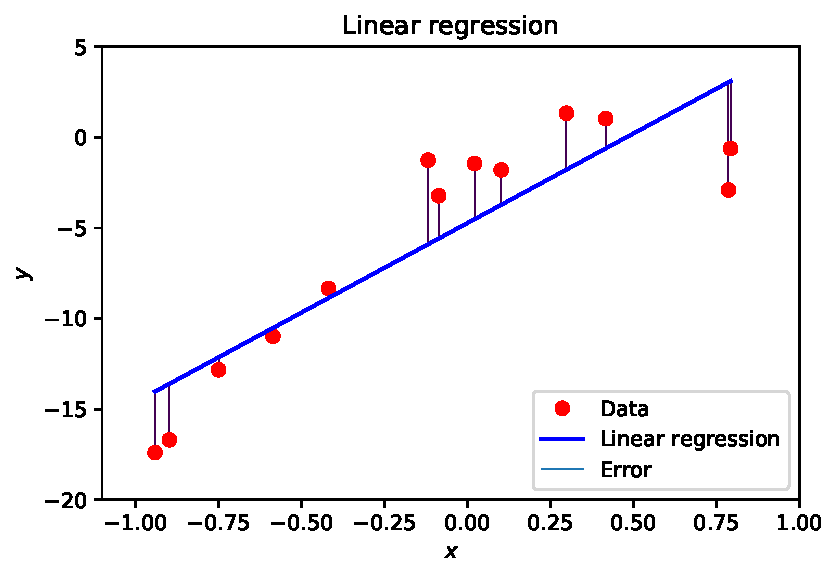
\includegraphics[width=0.31\textwidth]{../figures/week_1/linear_regression_error.pdf}
        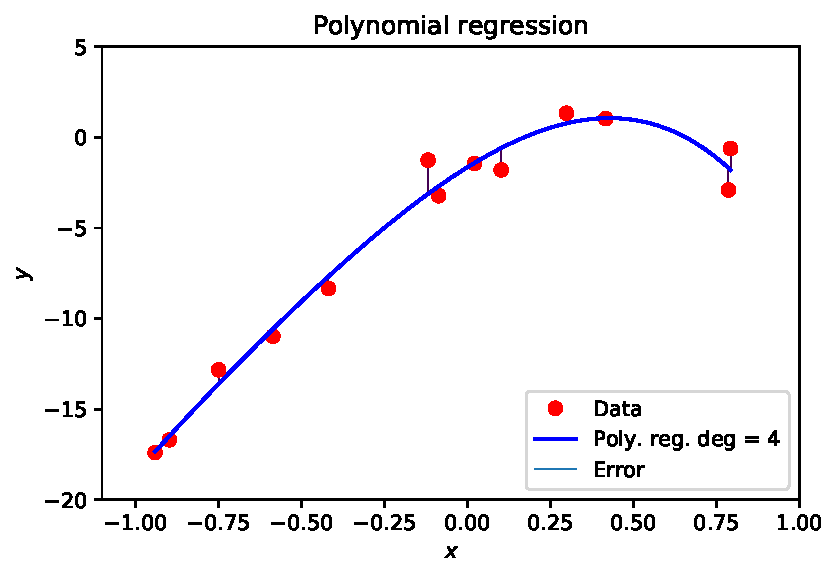
\includegraphics[width=0.31\textwidth]{../figures/week_1/polynomial_regression_degree_4.pdf}
        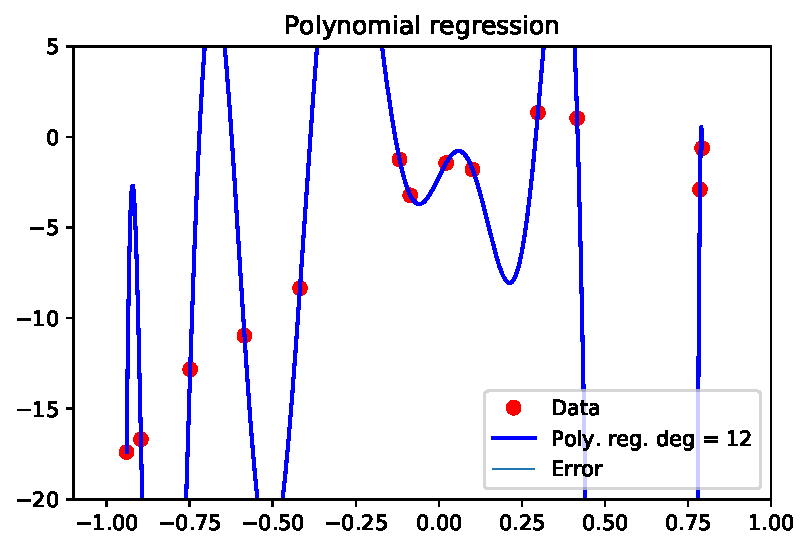
\includegraphics[width=0.31\textwidth]{../figures/week_1/polynomial_regression_degree_12.pdf}
    \end{center}
    \pause
    \begin{center}
        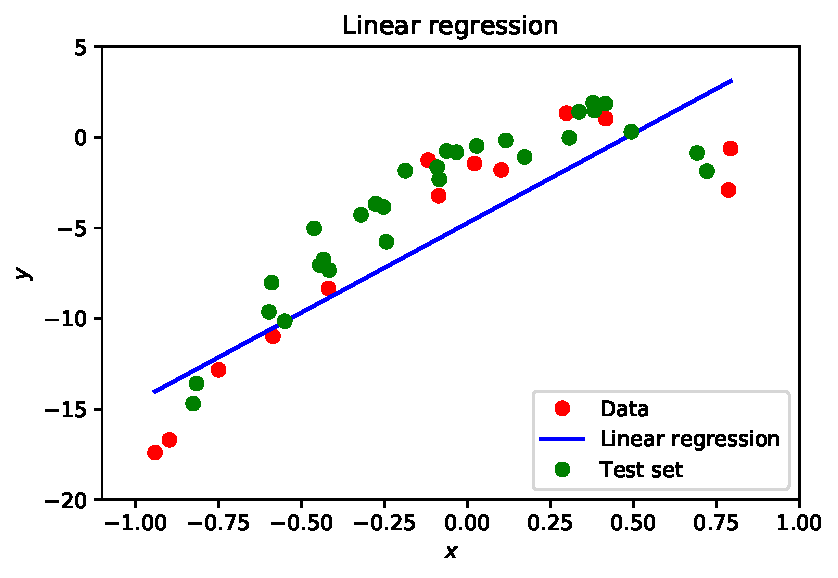
\includegraphics[width=0.31\textwidth]{../figures/week_1/linear_regression_test_set.pdf}
        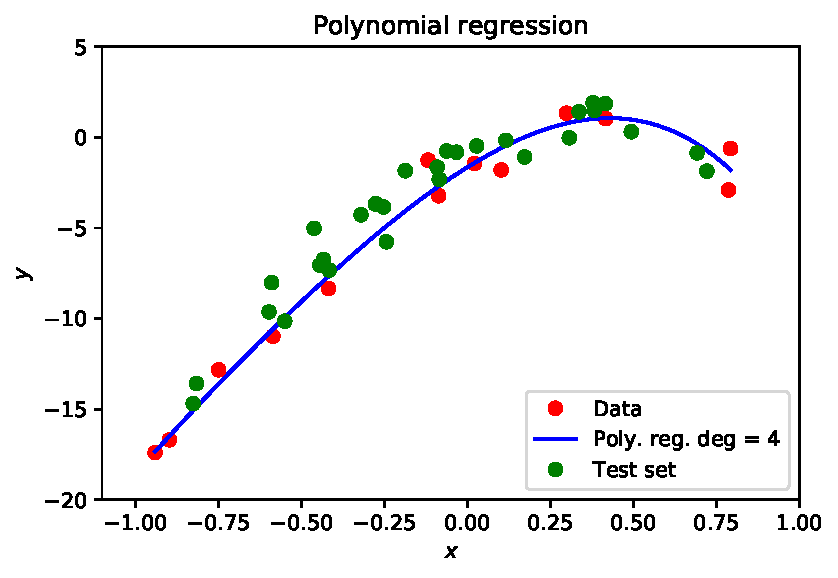
\includegraphics[width=0.31\textwidth]{../figures/week_1/polynomial_regression_degree_4_test_set.pdf}
        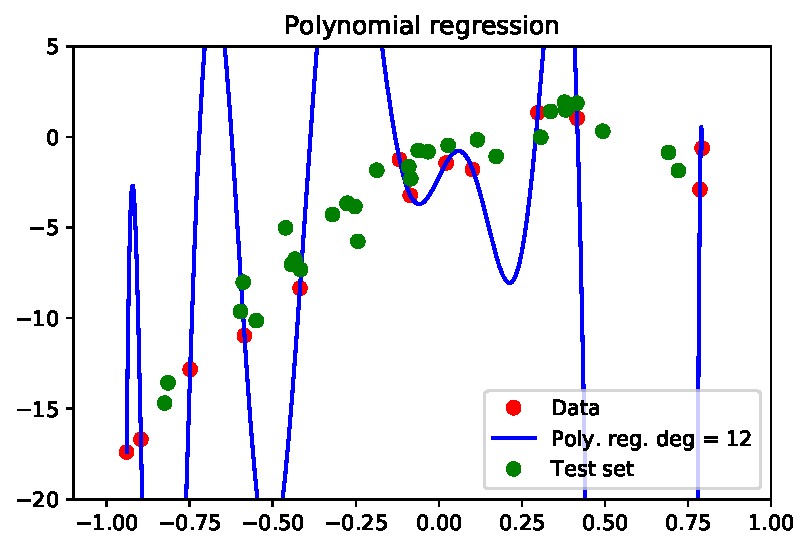
\includegraphics[width=0.31\textwidth]{../figures/week_1/polynomial_regression_degree_12_test_set.pdf}
    \end{center}
\end{frame}

\iffull
\begin{frame}
\frametitle{Overfitting and underfitting in polynomial estimation}
    \begin{itemize}
        \item Models with low capacity are not up to the task.
        \item Models with high-capacity can solve a complex task, but when the capacity is too high for the concrete (training) task there is the danger of overfitting.
        \item In our example: the linear function is unable to capture the curvature so it undefits.
        \item The degree-12 predictor is capable of fitting the training data, but it also able to find infinitely many functions that pass through the same points, so it has high probability of overfitting.
        \item The degree-4 function is the right solution and it generalizes well on the new data.
    \end{itemize}
\end{frame}
\fi

\begin{frame}
\frametitle{Generalization and capacity}
    \begin{itemize}
        \item Simpler functions generalize more easily, but we still need to choose a sufficiently complex hypothesis (function) to obtain small training error.
        \item Typically training error decreases with the increase of the model capacity until an (asymptotic) value is reached.
        \item The generalization error is U-shaped with the capacity range split in an underfitting and an overfitting zone\iffull (see next slide)\fi.
    \end{itemize}
\end{frame}


\begin{frame}
\frametitle{Generalization and capacity}
    \begin{center}
        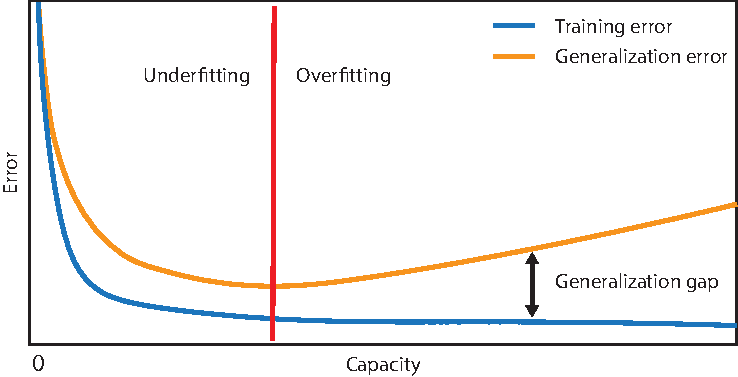
\includegraphics[width=0.85\textwidth]{../figures/week_1/generalization_gap.pdf}
    \end{center}
\end{frame}

\iffull
\begin{frame}
\frametitle{Training set size}
    \begin{itemize}
        \item Training and generalization error vary as the size of the training data set varies.
        \item Expected generalization error never increases as the size of the training set increases.
        \item Any fixed parametric model will asymptotically approach an error value that exceeds the so called Bayes error.
        \item It is possible for the model to have optimal capacity and still have a large gap between training and generalization errors.
        \item In that case the gap usually can be reduced with increasing the number of training examples.
    \end{itemize}
\end{frame}


\begin{frame}
\frametitle{Training set size}
    \begin{center}
        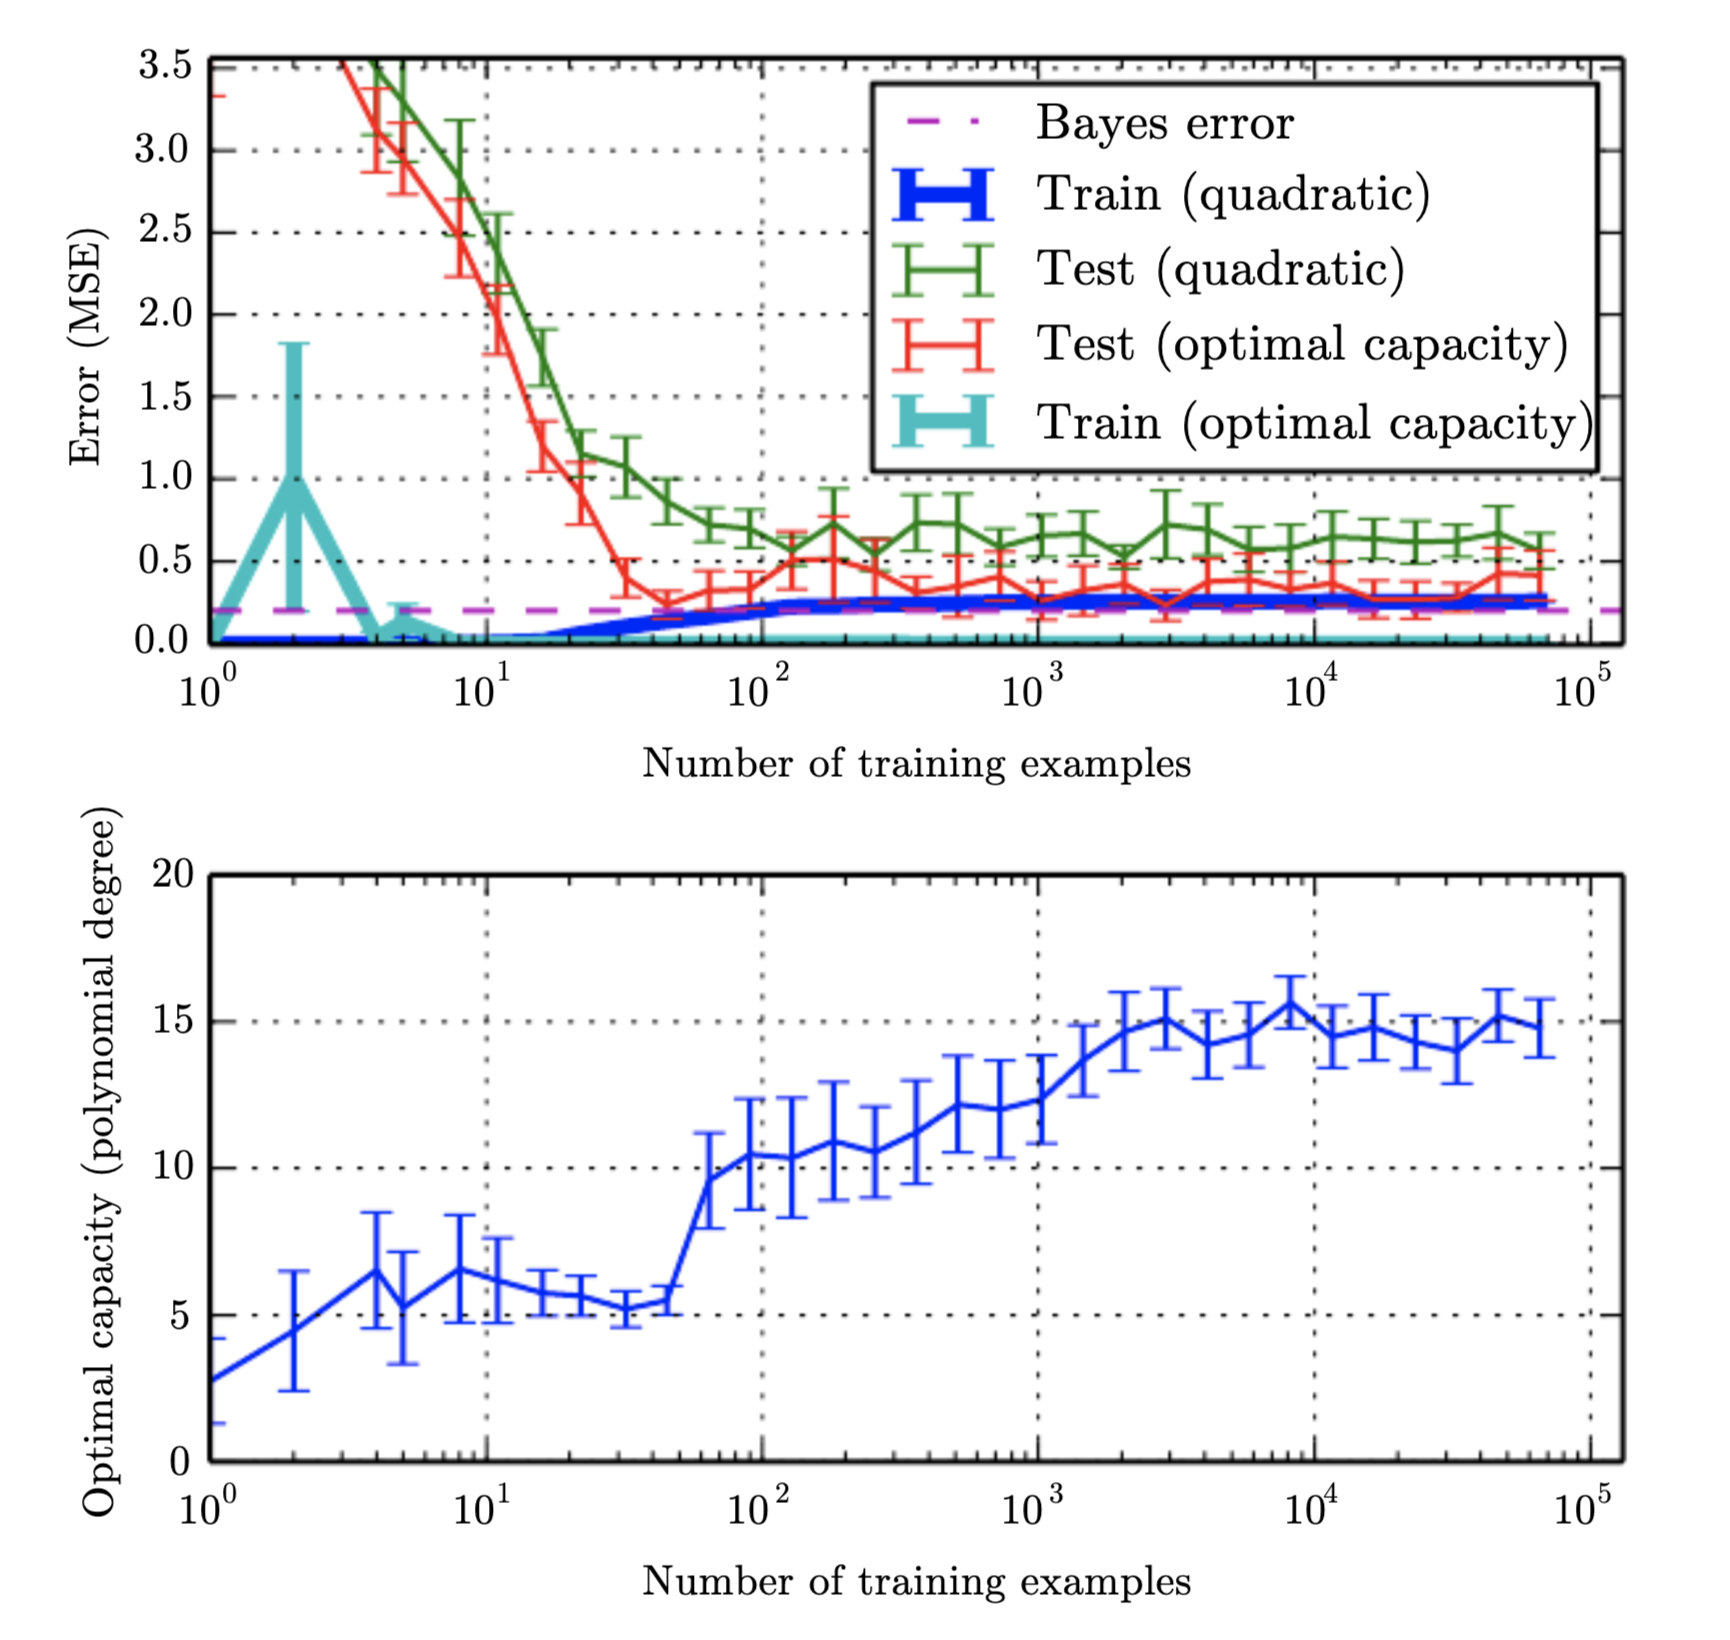
\includegraphics[width=0.7\textwidth]{../figures/week_1/training_set_size.png}
    \end{center}
    \tiny{Figure from \cite{deeplearning}}
\end{frame}
\fi


\iffull
\begin{frame}
\frametitle{The No Free Lunch theorem}
    \begin{itemize}
        \item {\bf No Free Lunch Theorem} for machine learning (Wolpert, 1996): \\
        Averaged over all possible data-generating distributions every classification algorithm has the same error rate when tested on new unobserved data.
        \item In some sense, no machine algorithm is universally better than any other algorithm.
        \item An interesting, but mainly theoretical result.
        \item In practice we often have an information about the probability distributions we deal with and can tailor our algorithms to perform well with particular distributions.
    \end{itemize}
\end{frame}
\fi 


\begin{frame}
\frametitle{Regularization}
    \begin{itemize}
        \item In addition to increasing and decreasing of the hypothesis space, i.e., the capacity, we can influence the learning algorithm by \textbf{giving preference to one solution over another in the hypothesis space}.
        \item In case both functions are eligible we can define a condition to express preference about one of the functions.
        \item The unpreferred solution is chosen only if it gives significantly better performance with the training data.
        \item \textit{More on regularization in the next lecture.}
    \end{itemize}
\end{frame}

\section{Model selection}

\begin{frame}
\frametitle{Model selection}
Materials:
\begin{itemize}
    \item Chapter I.5.3 from \cite{deeplearning}
\end{itemize}
\end{frame}

\begin{frame}
\frametitle{Hyperparameters and validation sets}
    \begin{itemize}
        \item {\bf Hyperparameters} are settings that can be used to control the behaviour of the algorithm.
        \item In general, the hyperparameters are not modified by the learning algorithm itself.
        \item {\bf Example}: In {\bf polynomial regression} the degree of the polynomial is a {\bf capacity} hyperparameter.
        \item A setting can be chosen to be hyperparameter when it is {\bf difficult to optimize} or - more often - when its derivation from the training set {\bf can lead to overfitting}.
        \begin{itemize}
            \item Example: in polynomial regression we can always fit the data better with a higher degree polynomial.
        \end{itemize}
    \end{itemize}
\end{frame}


\begin{frame}
\frametitle{Choice of training, validation, and test sets}
    \begin{itemize}
        \item The {\bf validation set} is used during training to predict the behaviour (generalization error) of the algorithm on new data, i.e., on the {test set} and to chose the hyperparameters.
        \item Ideally these two sets are disjoint.
        \item The validation set is chosen from the training data.
        \item The training data is split in two disjoint subsets.
        \iffull
        \item One subset is used to learn the parameters of the algorithm and the other is the validation set.
        \item The subset used to learn the parameters is still typically called a {\bf training set}.
        \fi
    \end{itemize}
\end{frame}

\iffull
\begin{frame}
\frametitle{Choice of training, validation, and test sets}
    \begin{itemize}
        \item Since the validation set is used to determine the hyperparameters it will typically underestimate the generalization error.
        \item However, it will usually better predict the generalization error than the training set.
        \item After the completion of the hyperparameters optimization we can estimate the generalization error using the test data.
        \item In practice the testing should be done also on different test data to avoid the test data becoming ``stale''.
    \end{itemize}
\end{frame}
\fi

\begin{frame}
\frametitle{Choice of training, validation, and test sets}
    \begin{center}
        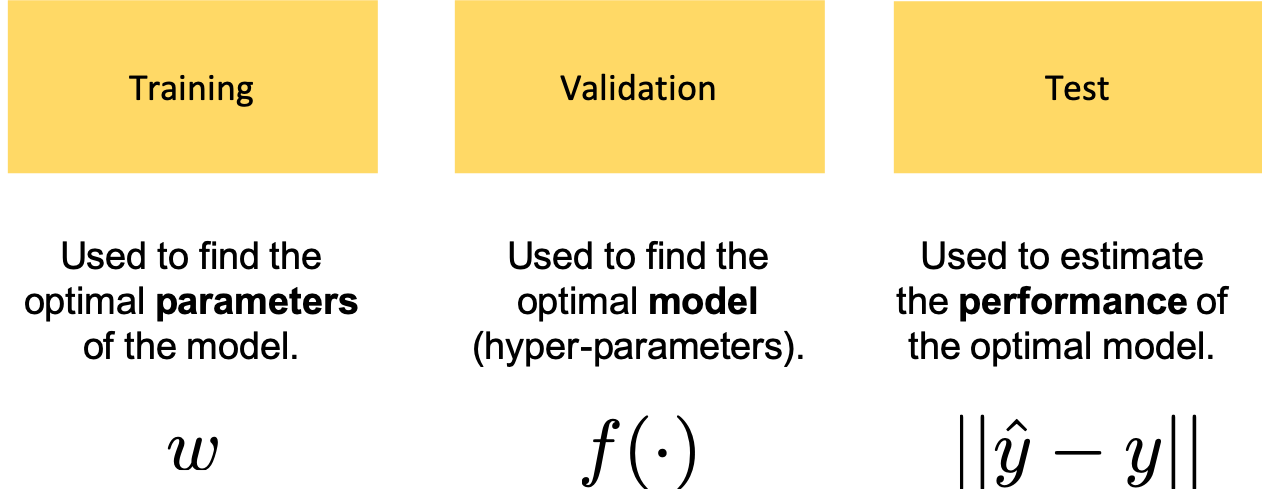
\includegraphics[width=0.95\textwidth]{../figures/week_1/subsets.png}
    \end{center}
\end{frame}

\iffull
\begin{frame}
\frametitle{Discussion point 4}
How large should the training, validation and testing datasets be as a percentage (\%) of the total available data?
\end{frame}
\fi

\begin{frame}
\frametitle{Cross-validation}
    \begin{itemize}
        \item Dividing the data set into disjoint training and test sets can result in a result in a too small validation and/or test set.
        \item In such cases all data is used to estimate the generalization error.
        \item We use procedures that repeat the training and testing on different randomly chosen subsets or splits of the original data set.
        \item The most common such procedure is the {\bf k-fold cross-validation}.
    \end{itemize}
\end{frame}

\iffull
\begin{frame}
\frametitle{Cross-validation}
    \begin{itemize}
        \item The original data is partitioned into $k$ (disjoint) subsets.
        \item The average error can be estimated by taking the average over $k$ trials.
        \item In trial $i$, the $i$-th subset is used as test set and the rest as training set.
        \item Problem: no unbiased estimators of the variance of such average error exist, but there are approximations that are used in practice.
    \end{itemize}
\end{frame}
\fi

\begin{frame}
\frametitle{Expectation (recap)}
\begin{itemize}
    \item The {\bf expectation} or {\bf expected} value of a function $f(x)$ with respect to a probability distribution $P(x)$ is the average value of $f$ over all values $x$ assuming they are drawn from $P$
$$\field{E}_{\text{x} \sim P} [f(x)] = \sum_{x} P(x) f(x)$$
$$\field{E}_{\text{x} \sim P} [f(x)] = \int p(x) f(x) dx$$
\end{itemize}

\end{frame}



\begin{frame}
\frametitle{Variance (recap)}
\begin{itemize}
    \item The {\bf variance} gives a measure of variation of the values of a random variable x $$\mbox{Var}(f(x)) = \field{E}[(f(x) - E[f(x)])^2]$$

\end{itemize}

\end{frame}

\section{Bias and variance trade-off}

\begin{frame}
\frametitle{Bias and variance trade-off}
Materials:
\begin{itemize}
    \item Chapter I.5.4 from \cite{deeplearning}
\end{itemize}
\end{frame}


\begin{frame}
\frametitle{Point estimation}
    \begin{itemize}
        \item For efficient design of learning algorithms it is useful to have formal characterizations of notions like generalization, overfitting and underfitting.
        \item To this end we introduce some definitions.
        \item {\bf Point estimation} is the attempt to provide the single "best" prediction of some quantity of interest.
        \item The quantity of interest can be a single parameter, parameter vector of some model, e.g., the weights $\vect{w}$ in the linear regression model.
        \iffull
        \item It can also be a whole function, e.g., the linear function or polynomial of some degree, like in the polynomial regression.
        \fi
    \end{itemize}
\end{frame}


\begin{frame}
\frametitle{Point estimation}
    \begin{itemize}
        \item Given a parameter $\vect{\theta}$ we denote its point estimate with ${\vect{\hat{\theta}}}$.
        \item As usual, let $\{\vect{x}^{(1)}, \ldots, \vect{x}^{(m)} \}$ be $m$ independent and identically distributed (i.i.d.) data points.
        \item A {\bf point estimator} or {\bf statistic} is any function of the data
        $$
        \hat{\vect{\theta}}_m = g(\vect{x}^{(1)}, \ldots, \vect{x}^{(m)}))
        $$
        \item This definition is very general. For instance, that the value returned by $g$ need not be close to the true value $\vect{\theta}$. Also $g$ might return a value which is outside the values that $\vect{\theta}$ is allowed to have.

    \end{itemize}
\end{frame}


\begin{frame}
\frametitle{Point estimation}
    \begin{itemize}
     \item Of course, a good estimator is still a function that returns values close to $\vect{\theta}$.
    \item Since the data is drawn from a random process, point estimate $\vect{\hat\theta}$ is considered to be a random variable and $\vect{\theta}$ is fixed, but unknown parameter.
    \end{itemize}
\end{frame}

\iffull
\begin{frame}
\frametitle{Function estimation}
    \begin{itemize}
         \item In {\bf function estimation}, we assume that there is a (true) function that describes the (approximate) relationship between $\vect{x}$ and $\vect{y}$
        $$\vect{y} = f(\vect{x}) + \vect{\epsilon}$$
        where $\vect{\epsilon}$ is the part of $\vect{y}$ which is not predictable from $\vect{x}$
        \item The goal is to find the {\bf function estimate} ({\bf model}) $\hat{f}$ which is a good approximation of $f$.
        \item The linear regression and polynomial regression can be seen both illustrate scenarios that can be interpreted as either estimating a parameter $\vect{w}$ or estimating a function $\hat{f}$.
    \end{itemize}
\end{frame}
\fi

\begin{frame}
\frametitle{Bias}
    \begin{itemize}
        \item A bias of an estimator $\vect{\hat{\theta}}_m$ is defined as
        $$
        \mbox{bias}(\vect{\hat{\theta}}_m) = \field{E}(\vect{\hat{\theta}}_m) - \vect{\theta}
        $$
        where the expectation is over the data and $\vect{\theta}$ is the true underlying value.
        \item An estimator $\vect{\hat{\theta}}_m$ is {\bf unbiased} if $\mbox{bias}(\vect{\hat{\theta}}_m) = 0$. Note that this implies $\field{E}(\vect{\hat{\theta}}_m) = \vect{\theta}$.
        \item $\vect{\hat{\theta}}_m$ is {\bf asymptotically unbiased} if $\lim_{m \rightarrow \infty} \mbox{bias}(\vect{\hat{\theta}}_m) = 0$ \\
        (implying $\lim_{m \rightarrow \infty} \field{E}(\vect{\hat{\theta}}_m) = \vect{\theta}$).
    \end{itemize}
\end{frame}


\begin{frame}
\frametitle{Bias: example}
    \begin{itemize}
        \item {\bf Example}: Consider samples $\{x^{(1)}, \ldots, x^{(m)}\}$ i.i.d distributed according to the Gaussian distribution
        $$
        p(x^{(i)};\mu, \sigma^2) = \frac{1}{\sqrt{2 \pi \sigma^2}} \exp \left ( -\frac{1}{2} \frac{x^{(i)} - \mu}{\sigma^2} \right )
        $$
        \item The {\bf sample mean} is a common estimator of the Gaussian mean parameter
        $$
        \hat{\mu}_m = \frac{1}{m} \sum_{i=1}^{m}x{(i)}
        $$
    \end{itemize}
\end{frame}


\begin{frame}
\frametitle{Bias: example}
    We compute the bias as expectation by substituting the Gaussian distribution in the formula
    \begin{eqnarray*}
    \mbox{bias}(\mu_m) =  & \field{E}[\mu_m] - \mu  \\
     = & \field{E} \left [   \frac{1}{m} \sum_{i=1}^{m }x^{(i)} \right ] - \mu \\
     = & \left (   \frac{1}{m} \sum_{i=1}^{m} \field{E}[x^{(i)}] \right ) - \mu \\
     = & \left (   \frac{1}{m} \sum_{i=1}^{m} \mu \right ) - \mu \\
     = & \mu - \mu = 0
    \end{eqnarray*}
    The sample mean is an unbiased estimator of Gaussian mean parameter.
\end{frame}



\begin{frame}
\frametitle{Bias: example}
    \begin{itemize}
        \item {\bf Example}: Estimators of the variance of a Gaussian distribution
        \item We compare two different estimators of the variance $\sigma^2$ parameter
        \item {\bf Sample variance}
        $$
        \hat{\sigma}^2 = \frac{1}{m}\sum_{1}^{m} \left (  x^{(i)} - \hat{\mu}_m \right )^2
        $$
        where $\hat{\mu}$ is the sample mean.
        \item We are interested in computing
        $$
        \mbox{bias}(\hat{\sigma}^2_m) = \field{E} [\hat{\sigma}^2_m] - \sigma^2
        $$
    \end{itemize}
\end{frame}


\begin{frame}
\frametitle{Bias: example}
\begin{itemize}
    \item First we evaluate $\field{E} [\hat{\sigma}^2_m]$:
    $$
    \field E [\hat{\sigma}^2_m] = \field{E} \left [ \frac{1}{m}\sum_{1}^{m} \left (  x^{(i)} - \hat{\mu}_m \right )^2 \right ] = \frac{m-1}{m} \sigma^2
    $$
    \item Back to the bias
    $$
    \mbox{bias}(\hat{\sigma}^2_m) = \field{E} [\hat{\sigma}^2_m] - \sigma^2  = \frac{m-1}{m} \sigma^2 - \sigma^2 = -\frac{\sigma^2}{m}
    $$
    \item Therefore the sample variance is a \textbf{biased} estimator.
\end{itemize}
\end{frame}


\begin{frame}
\frametitle{Bias: example}
\begin{itemize}
    \item The {\bf unbiased variance estimator} is defined as


    $$
        \tilde{\sigma}^2 = \frac{1}{m - 1}\sum_{1}^{m} \left (  x^{(i)} - \hat{\mu}_m \right )^2
    $$
    \item Indeed
    $$
    \field E [\tilde{\sigma}^2_m] = \field{E} \left [ \frac{1}{m-1}\sum_{1}^{m} \left (  x^{(i)} - \hat{\mu}_m \right )^2 \right ] = \frac{m-1}{m-1} \sigma^2 = \sigma^2
    $$
    and the bias is $0$. \\
\end{itemize}
\end{frame}


\begin{frame}
\frametitle{Variance and standard error}
    \begin{itemize}
        \item Another important feature of an estimator is its variance.
        \item The {\bf variance} of an estimator is simple its statistical variance $\mbox{Var}(\hat{\theta})$ over the training set as a random variable.
        \item Alternatively we can compute the {\bf standard error} (the square root of the variance) $\mbox{SE}(\hat{\theta)}$.
        \item The variance or the standard error provide a measure how much the estimate would vary as we resample the data independently from the underlying data generating process.
        \item We would prefer a relatively low variance of the estimator.
    \end{itemize}
\end{frame}


\begin{frame}
\frametitle{Variance and standard error}
    \begin{itemize}
        \item The standard error of the mean estimator is given as
        $$
        \mbox{SE}(\hat{\mu}) = \sqrt{\mbox{Var}\left[\frac{1}{m}\sum_{i=1}^m x^{(i)}\right]} = \frac{\sigma}{\sqrt{m}}
        $$
        where $\sigma$ is the true variance of the distribution, i.e., the samples $x^{(i)}$.
        \item Neither the square root of the sample variance nor the square root of the unbiased estimator of the variance give an unbiased estimate of the standard deviation.
        \item Both approaches underestimate the true standard deviation.
        \item However, for large $m$ the approximation works quite well.
    \end{itemize}
\end{frame}


\begin{frame}
\frametitle{Variance and standard error}
    \begin{itemize}
        \item In machine learning the generalization error is estimated based on the sample mean of the error on the test set.
        \item The accuracy of the estimate depends on the number of the examples.
        \item From the statistical theory (central limit theorem) we know that the mean is distributed with normal distribution for which we can establish confidence intervals.
        \item For instance, the 95\% confidence interval is given by
        $$
        \left [ \hat{\mu_m} - 1.96 \mbox{SE}(\hat{\mu}_m), \hat{\mu_m} + 1.96 \mbox{SE}(\hat{\mu}_m \right ]
        $$
        \item Then we can say that algorithm A is better than algorithm B of the confidence upper bound for the error of A is less than the corresponding lower bound of B.
    \end{itemize}
\end{frame}


\begin{frame}
\frametitle{Trading off bias and variance to minimize  mean squared error}
    \begin{itemize}
        \item Bias and variance measure two different sources of error in an estimator.
        \item Bias measures the expected deviation with the true value of the estimator.
        \item Variance provides a measure of the deviation from the expected value of the estimator depending on the particular data sampling.
    \end{itemize}
\end{frame}


\begin{frame}
\frametitle{Trading off bias and variance to minimize  mean squared error}
    \begin{itemize}
        \item Often we need to make a trade-off between these two.
        \item The most common way to do this is via cross-validation.
        \item An alternative is to compare the {\bf mean squared error} (MSE) of the estimates.
        $$
        \mbox{MSE} = \field{E}[(\hat{\theta}_m -  \theta)^2] = \mbox{bias}(\hat{\theta}_m)^2 + \mbox{Var}(\hat{\theta}_m)
        $$
        \item The smaller MSE the better - so minimizing both the bias and variance is always preferable.

    \end{itemize}
\end{frame}


\begin{frame}
\frametitle{Bias and variance}
    \begin{itemize}
        \item Our original goal was to provide a mathematical support for the notions of capacity, underfitting, and overfitting.
        \item Indeed there is a close relationship between these three concepts and bias and variance.
        \item When generalization error is measured by MSE (and hence indirectly via bias and variance) increasing capacity tends to increase variance and decrease bias.
        \item Again the generalization as a function of capacity is given by an U-shaped curve.
    \end{itemize}
\end{frame}

\begin{frame}
\frametitle{Discussion}
How will the estimated regression model change when one training data point is replaced with another one?
\vfill
  \begin{center}
        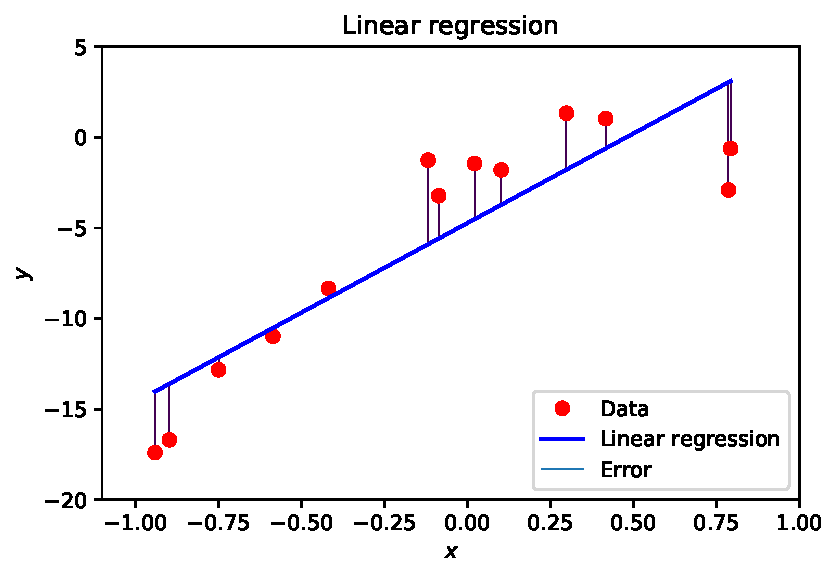
\includegraphics[width=0.31\textwidth]{../figures/week_1/linear_regression_error.pdf}
        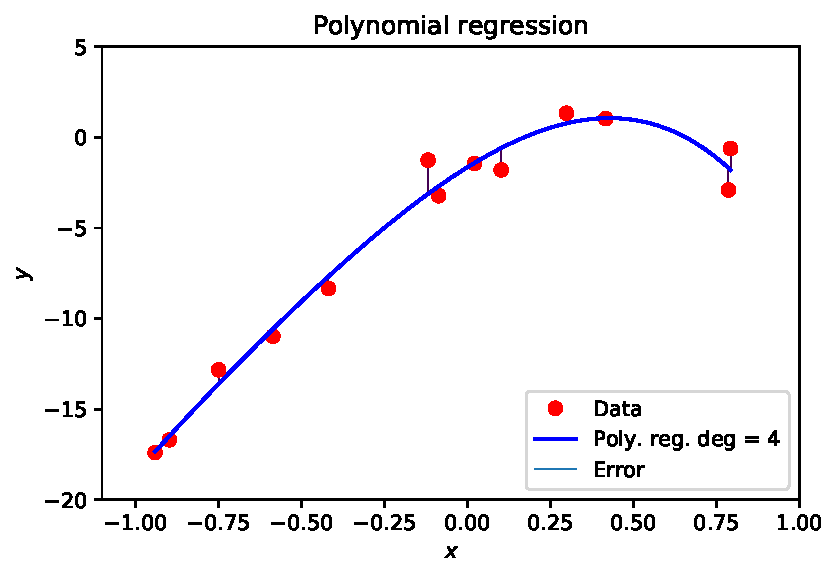
\includegraphics[width=0.31\textwidth]{../figures/week_1/polynomial_regression_degree_4.pdf}
        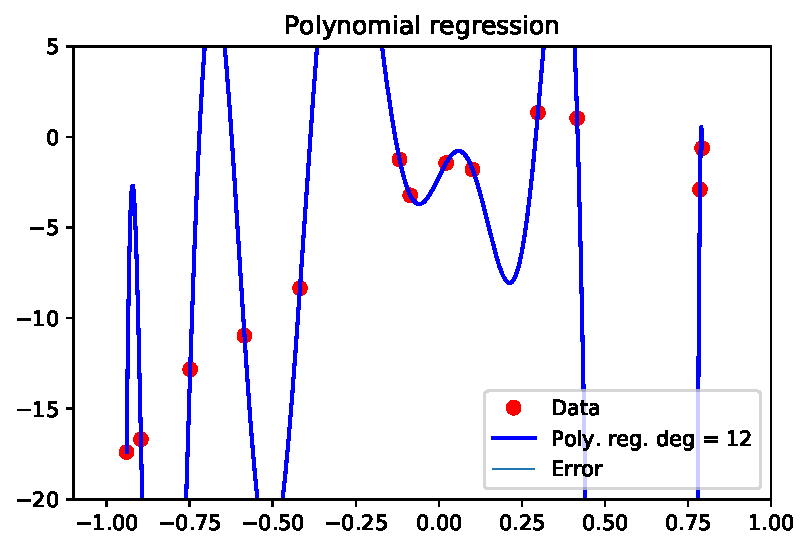
\includegraphics[width=0.31\textwidth]{../figures/week_1/polynomial_regression_degree_12.pdf}
    \end{center}
  
\end{frame}

\begin{frame}
\frametitle{Bias and variance}
    \begin{center}
        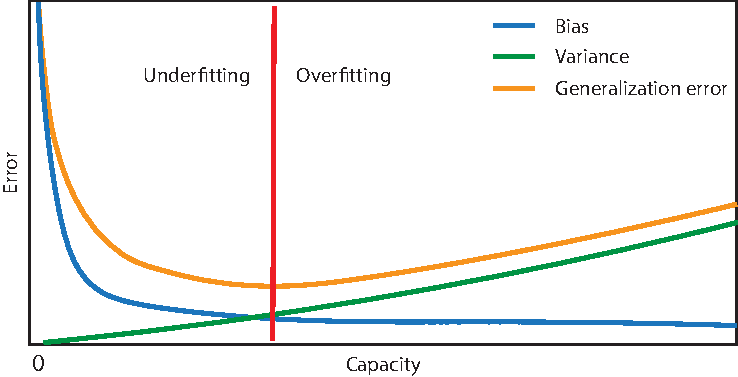
\includegraphics[width=0.85\textwidth]{../figures/week_1/bias_variance.pdf}
    \end{center}
\end{frame}

\iffull
\begin{frame}
\frametitle{Consistency}
    \begin{itemize}
        \item So far we considered fixed size of the training data sets.
        \item We expect that as the number $m$ of training examples grows the estimators will converge to the true value of the parameters.
        \item More formally this is captured in the notion of {\bf consistency}
        $$
        \mbox{plim}_{m \rightarrow \infty} \hat{\theta}_m = \theta
        $$
        where $ \mbox{plim}$ denotes convergence in probability: for any $\epsilon > 0$, $P(\mid \hat{\theta}_m - \theta \mid > \epsilon) \rightarrow 0$ as $m \rightarrow \infty$.
        \item For consistent models the bias decreases as $m$ increases, however a decreasing bias (when $m$ increases) does not imply consistency.
    \end{itemize}
\end{frame}
\fi

\iffull % Maximum likelihood estimation

\section{Maximum likelihood estimation}

\begin{frame}
\frametitle{Maximum likelihood estimation}
Materials:
\begin{itemize}
    \item Chapter I.5.5 from \cite{deeplearning}
\end{itemize}
\end{frame}

\begin{frame}
\frametitle{Maximum likelihood estimation}
    \begin{itemize}
        \item We would like to have some principle from which we can derive good estimator functions for a large scale of models.
        \item The {\bf maximum likelihood estimation} is the most common such principle.
        \item Given observation data and a corresponding (statistical) model our goal is to find the parameter vector which imply the highest probability to obtain the data.
    \end{itemize}
\end{frame}


\begin{frame}
\frametitle{Maximum likelihood estimation}
    \begin{itemize}
        \item Consider a set of $m$ examples $\field{X} = \{ \vect{x}^{(1)}, \vect{x}^{(2)}, \ldots,  \vect{x}^{(m)} \}$ drawn independently from the true but unknown distribution $p_{\mbox{data}}(\text{\bf x})$.
        \item Let $p_{\mbox{model}}(\text{\bf x};\vect{\theta})$ be a parametric family of probability distributions, i.e., for each $\vect{\theta}$ we get a different distribution  $p_{\mbox{model}}$.
        \item $p_{\mbox{model}}(\vect{x};\vect{\theta})$ maps any configuration $\vect{x}$ to a real number estimating the (true) probability $p_{\mbox{data}}(\vect{x})$
    \end{itemize}
\end{frame}


\begin{frame}
\frametitle{Maximum likelihood estimation}
    \begin{itemize}
        \item The maximum likelihood estimator for $\vect{\theta}$ is then defined as
        $$
        \vect{\theta}_{\mbox{ML}} = \mbox{argmax}_{\vect{\theta}} p_{\mbox{model}}(\field{X};\vect{\theta}) =  \mbox{argmax}_{\vect{\theta}} \prod_{i = 1}^{m} p_{\mbox{model}}(\vect{x}^{(i)};\vect{\theta})
        $$
        Note that also the empirical distribution $\hat{p}_{\mbox{data}}$ is implicitly present in the formula through $\vect{x}^{(i)}$.
        \item A more convenient equivalent optimization problem is obtained by taking logarithm of the product
        $$
        \vect{\theta}_{\mbox{ML}} = \mbox{argmax}_{\vect{\theta}} p_{\mbox{model}}(\field{X};\vect{\theta}) = \sum_{i=1}^{m} \log p_{\mbox{model}}\vect{x}^{(i)};\vect{\theta})
        $$
    \end{itemize}
\end{frame}


\begin{frame}
\frametitle{Maximum likelihood estimation}
    \begin{itemize}
        \item We can further rescale by dividing the expression by $m$
        $$
        \vect{\theta}_{\mbox{ML}} = \mbox{argmax}_{\vect{\theta}} p_{\mbox{model}}(\field{X};\vect{\theta}) 
        $$
        $$
        \vect{\theta}_{\mbox{ML}} =  \mbox{argmax}_{\vect{\theta}} \field{E}_{\text{\bf x} \sim  \hat{p}_{\mbox{data}}} \log p_{\mbox{model}}(\vect{x};\vect{\theta})
        $$
        \item In this way the problem is expressed as an equivalent expectation problem (now the empirical distribution $\hat{p}_{\mbox{data}}$ becomes explicit).
    \end{itemize}
\end{frame}


\begin{frame}
\frametitle{Maximum likelihood estimation}
    \begin{itemize}
        \item Perhaps more straightforwardly, the maximum likelihood estimation can be seen as minimizing the dissimilarity between $\hat{p}_{\mbox{data}}$ and $p_{\mbox{model}}$.
        \item The degree of dissimilarity is given by the KL-divergence
        $$
        D_{\mbox{KL}} (\hat{p}_{\mbox{data}} \lVert p_{\mbox{model}}) = \field{E}_{\text{\bf x} \sim  \hat{p}_{\mbox{data}}} [\log \hat{p}_{\mbox{data}}(\vect{x}) - \log p_{\mbox{model}}(\vect{x})]
        $$
        \item Only the term of the right is function of the model, so it is the only one which needs to be minimized
        $$
        - \field{E}_{\text{\bf x} \sim  \hat{p}_{\mbox{data}}} [\log p_{\mbox{model}}(\vect{x})]
        $$
        which is equivalent with the maximization problem from the previous slide.
        \item It boils down to minimizing the {\bf cross-entropy} between the two distributions.
    \end{itemize}
\end{frame}


\begin{frame}
\frametitle{Maximum likelihood estimation}
    \begin{itemize}
        \item {\bf The maximum likelihood estimation can be seen as an attempt to make the model distribution } $p_{\mbox{model}}$ {\bf to match the empirical distribution} $\hat{p}_{\mbox{data}}$.
        \item Ideally we would like to match the data generating distribution $p_{\mbox{data}}$, but we do not have access to it.
    \end{itemize}
\end{frame}


\begin{frame}
\frametitle{Conditional log likelihood and mean square error}
    \begin{itemize}
        \item The maximal likelihood estimator can be generalized to estimate a conditional probability $P(\text{\bf y} \mid \text{\bf x} ; \vect{\theta})$ .
        \item Let all inputs be given by $\vect{X}$ and all observed outputs by $\vect{Y}$. Then the conditional maximum likelihood estimator is
        $$
        \vect{\theta_{\mbox{ML}}} = \mbox{arg max}_{\theta} P(\vect{Y} \mid \vect{X}; \vect{\theta})
        $$
        \item If the examples are assumed to be i.i.d., then this can be decomposed into
        $$
        \vect{\theta_{\mbox{ML}}} = \mbox{arg max}_{\theta} \sum_{i=1}^{m} \log P(\vect{y}^{(i)} \mid \vect{x}^{(i)}; \vect{\theta})
        $$
    \end{itemize}
\end{frame}

\iffull
\begin{frame}
\frametitle{Example: linear regression as maximum likelihood}
    \begin{itemize}
        \item The linear regression seen as an algorithm that learns to take an input $\vect{x}$ and produce output $\hat{y}$.
        \item This function from $\vect{x}$ to $\hat{y}$ is chosen to minimize the mean squared error.
        \item This criterion was introduced more or less arbitrarily.
        \item We revisit linear regression from the point of view of maximal likelihood.
        \item We think of the model as producing a conditional distribution $p(y \mid \vect{x})$ instead of a single prediction $\hat{y}$.
    \end{itemize}
\end{frame}
\fi

\begin{frame}
\frametitle{Example: linear regression as maximum likelihood}
    \begin{itemize}
        \item With an infinitely large training set we might see several examples whit the same input $\vect{x}$ but different $y$.
        \item The learning algorithm needs to fit the distribution to all these $y$ corresponding to the same $\vect{x}$.
        \item To derive the linear regression algorithm we assume $p(y \mid \vect{x}) = \mathcal{N}(y; \hat{y}(\vect{x};\vect{w}), \sigma^2)$, where $\hat{y}(\vect{x};\vect{w})$ gives the (prediction of the) mean of the normal distribution and $\sigma$ is fixed to some chosen constant.
        \item The parameter vector $\theta$ corresponds in this case to $\vect{w}$.
    \end{itemize}
\end{frame}

\begin{frame}
\frametitle{Example: linear regression as maximum likelihood}
    \begin{itemize}
        \item By substituting (the full Gaussian function version of) $p(y \mid \vect{x})$ in the conditional log-likelihood formula we obtain
        $$
        \sum_{i=1}^{m} \log p(\vect{x}^{(i)} \mid y^{(i)}; \vect{\theta}) =
        -m \log \sigma - \frac{m}{2} \log(2\pi) - \sum_{i=1}^{m }\frac{\norm{\hat{y}^{(i)} - y^{(i)}}^2}{2 \sigma^2}
        $$
        where $\hat{y}^{(i)}$ is the linear regression on the $i$-th input $\vect{x}^{(i)}$.
        \item By comparing with the mean squared error
        $$
           \mbox{MSE}_{\mbox{train}} = \frac{1}{m} \sum_{i=1}^{m} \norm{\hat{y}^{(i)} - y^{(i)}}^2
        $$
        one can see that maximizing the log-likelihood with respect to $\vect{w}$ results with the same estimate of $\vect{x}$ as minimizing MSE. \iffull {\small (The third term in the log-likelihood forumula, needs to be as small as possible.)} \fi
    \end{itemize}
\end{frame}

\iffull
\begin{frame}
\frametitle{Properties of maximum likelihood}
    \begin{itemize}
        \item It can be shown that the maximum likelihood estimator is the best asymptotically, i.e. as $m \rightarrow \infty$, in terms of its convergence rate.
        \item {\bf Property of consistency}: as the number of training examples approaches infinity the maximum likelihood estimate of a parameter converges towards the true parameter value.
        \item The maximum likelihood estimator has the property of consistency provided:
            \begin{itemize}
                \item The true distribution $p_{\mbox{data}}$ is in the model family
                $p_{\mbox{model}}(\cdot; \vect{\theta})$ %\\
                %(otherwise no estimator can recover $p_{\mbox{data}}$)
                \item $p_{\mbox{data}}$ corresponds to exactly one value of $\vect{\theta}$ \\
                %(Otherwise, although $p_{\mbox{data}}$ might be recovered, it is not possible to dtermine which value of $\thata$ was used in the generate the data)
            \end{itemize}
    \end{itemize}
\end{frame}
\fi

\fi %Maximum likelihood estimation

\iffull % Model evaluation

\section{Model evaluation}

\begin{frame}
\frametitle{Model evaluation}
Materials:
\begin{itemize}
    \item \cite{ROC}
\end{itemize}
\end{frame}


\begin{frame}
\frametitle{Model evaluation}
    \begin{itemize}
        \item To quantitatively evaluate a machine learning algorithm we need to define a {\bf performance measure}.
        \item Usually the performance measure is specific to the task carried out by the algorithm.
        \item For classification tasks a natural measure is the model {\bf accuracy}.
        \item The {\bf accuracy} is defined as the proportion of examples for which the model produces the correct output.
        \item An equivalent (complementary) measure is the {\bf error rate} defined as the proportion of incorrect outputs.
    \end{itemize}
\end{frame}

\begin{frame}{Model evaluation}
    \begin{itemize}
        \item The best way to evaluate a machine learning algorithm is by applying it to a {\bf test set} data which has not been seen before.
        \item Ideally there should be {\bf no overlap} between the {\bf test set} and  the {\bf training set} used to obtain the model.
    \end{itemize}
\end{frame}

\begin{frame}\frametitle{Binary classification}
    \begin{itemize}
        \item We consider {\bf binary classification} problems, i.e., problems using only two classes/
        \item Formally each input example $x^{(i)}$ needs to be mapped into one element of the set $\{\vect{p},\vect{n}\}$ of {\bf true} classes.
        \item A {\bf classification model} ({\bf classifier}) is a function from the input examples to the set $\{\vect{Y}, \vect{N}\}$ of {\bf predicted classes} or {\bf hypothesized classes}.
        \item $\vect{p},\vect{n}$ correspond to $\vect{Y},\vect{N}$, respectively.
    \end{itemize}
\end{frame}


\begin{frame}\frametitle{Binary classification}
    \begin{itemize}
        \item For a given classifier there are four possible outcomes.
        \item If the true class of $x^{(i)}$ is $\vect{p}$ and the predicted class is $\vect{Y}$ then we have a {\bf true positive} (TP); if it was classified $\vect{N}$, then we have a {\bf false negative} (FN).
        \item Symmetrically, a  $x^{(i)}$ with true class $\vect{n}$ which is assigned a predicted class $\vect{N}$ is a {\bf true negative} (TN); if the predicted class is $\vect{Y}$, then it is a false positive (FP).
    \end{itemize}
\end{frame}


\begin{frame}
\frametitle{Confusion matrix}
     These four combinations can be put together in a {\bf confusion matrix}, also called {\bf contingency table}.
     \begin{table}[Confusion Matrix]
            \begin{tabular}{c|c|c|c|}
            \multicolumn{2}{c}{} & \multicolumn{2}{c}{True class} \\
            \cline{3-4}
            \multicolumn{2}{c|}{} & $\vect{p}$ & $\vect{n}$ \\
            \cline{2-4}
            \multirow{6}{*}{Predicted class} & \multirow{3}{*}{$\vect{Y}$} &  True & False  \\
                &   & positives & positives  \\
                &   & (TP) & (FP) \\
            \cline{2-4}
                & \multirow{3}{*}{$\vect{N}$} & False &  True  \\
                &   &  negatives & negatives  \\
                &   & (FN) & (TN) \\
            \cline{2-4}
            \end{tabular}
        \end{table}
\end{frame}



\begin{frame}
 \frametitle{Binary classifications metrics}
    \begin{itemize}
        \item Using the four basic categories of prediction outcomes (TP, FP, TN, FN) we can derive various {\bf  measures} of performance of classification models.
        \item For instance the accuracy can be defined as
        $$\mbox{Accuracy} = \frac{TP+TN}{TP+FP+TN+FN}$$
        \item Also quite frequently used measures are \\

    \end{itemize}
    \small{
        $$Sensitivity = \frac{TP}{TP+FN} \hspace{1em} Specificity = \frac{TN}{TN+FP} \hspace{1em} Precision = \frac{TP}{TP+FP}$$
        }
\end{frame}


\begin{frame}
\frametitle{Binary classification metrics}
    \begin{itemize}
        \item Sensitivity is also called {\bf recall}, {\bf true positive rate} or {\bf hit rate}.
        \item In medical contexts the sensitivity can be interpreted as a measure of the extent to which diseased individuals are correctly diagnosed.
        \item In general: measures the proportion of the target group the method is able to detect, i.e. how sensitive is to this group.
        \item Specificity is also called {\bf true negative rate} or {\bf selectivity}.
        \item In medical contexts the specificity can be interpreted as a measure of the extent to which healthy individuals are correctly diagnosed.
        \item The precision tells us which proportion of the positive predictions is correct.
    \end{itemize}
\end{frame}

\begin{frame}
\frametitle{Discussion point 6}
You have developed a method for some image analysis diagnostic task that has very high sensitivity (e.g. 0.99) but relatively low specificity (e.g. 0.25). 

Can this be still a useful tool for clinicians and if so in what context? \end{frame}

\begin{frame}
\frametitle{Binary classification metrics}
    \begin{itemize}
        \item Sometimes the above mentioned measures are not sufficient.
        \item For example, in a population in which the percentage of healthy individuals is much larger than the diseased individuals, it is easy to achieve high specificity by trivially classifying each patient as healthy.
        \item We can obtain more objective evaluation by combing metrics.
        \item The metrics $F_1$ is the harmonic mean (average) of the precision and recall (sensitivity)
        $$
        \frac{2}{F_1} = \frac{1}{Precision}+\frac{1}{Recall} \text{  or  } F_1 = 2 \cdot \frac{Precision \cdot Recall}{Precision+Recall}
        $$
    \end{itemize}
\end{frame}

\begin{frame}
\frametitle{Areas under the curve measures}
    \begin{itemize}
        \item (Binary) classifications often depend on some parameter (e.g., threshold).
        \item Hence on way to combine two metrics is by assigning them to the axes of a coordinate system and varying this parameter to construct a graphical plot.
        \item We obtain a curve (actually, most of the time series of points) such that each point corresponds to a particular parameter value.
        \item The area under the curve is a measure of how good is the classification.
    \end{itemize}
\end{frame}


\begin{frame}
\frametitle{Receiver Operating Characteristic (ROC) curve}
    \begin{itemize}
        \item The ROC curve plots the true positive rate (sensitivity) versus the false positive rate (1 - specificity).
        \begin{center}
        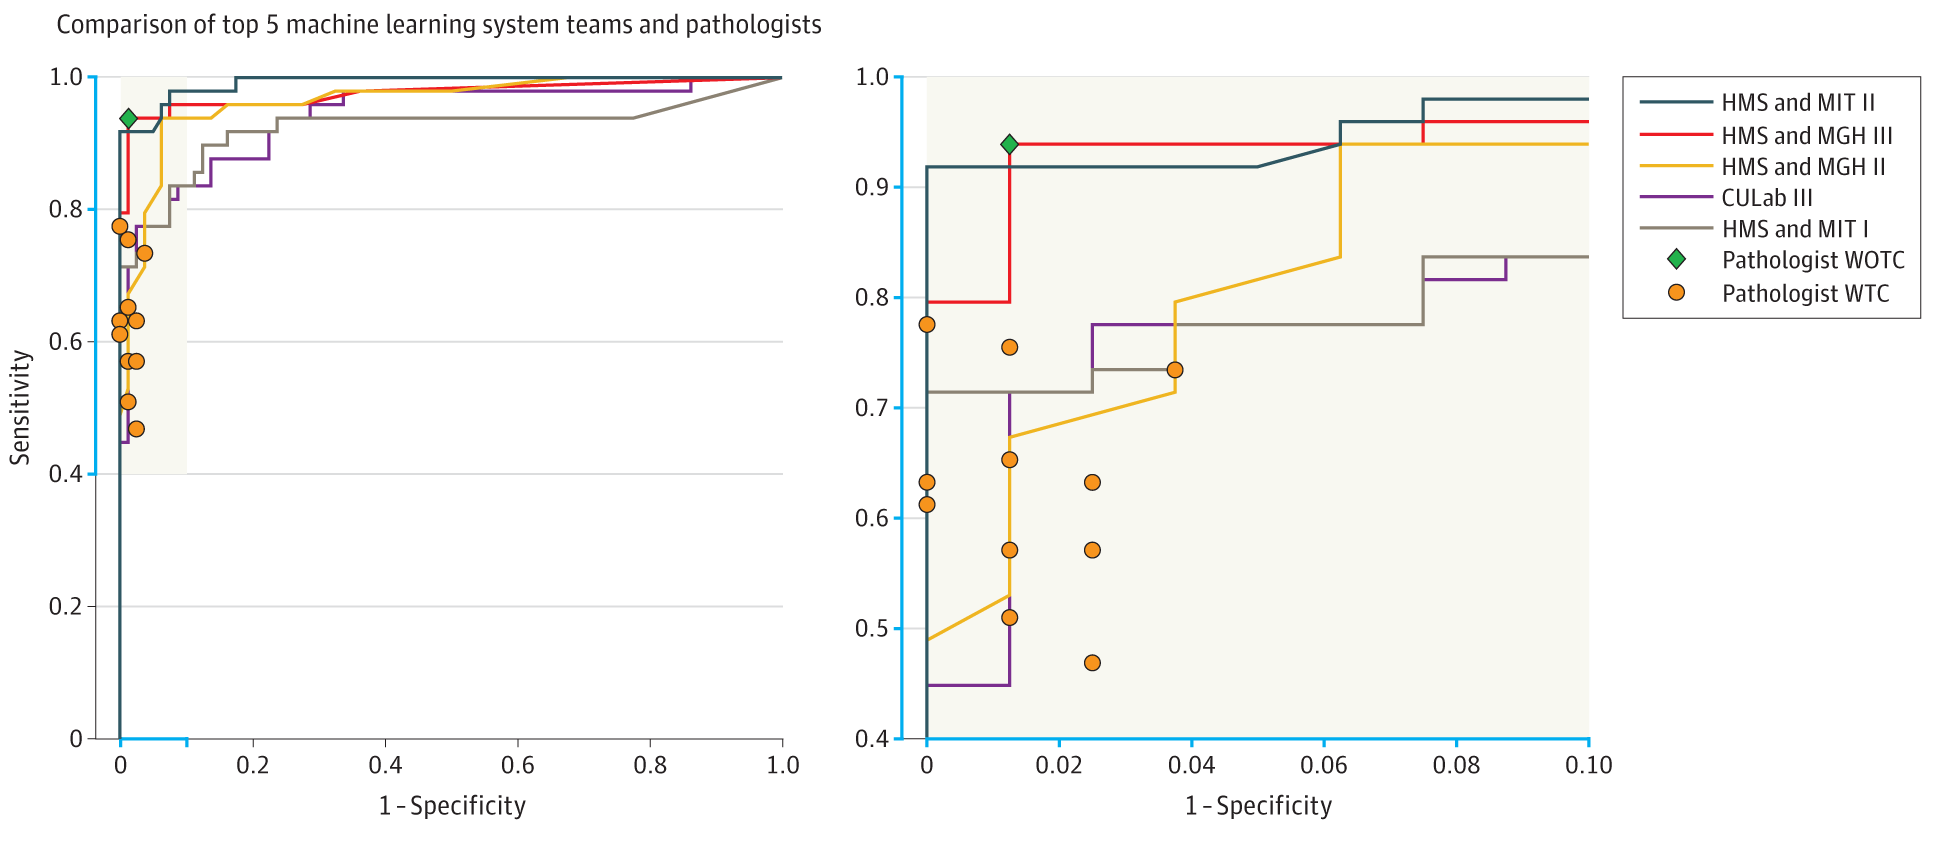
\includegraphics[width=0.95\textwidth]{../figures/week_1/camelyon_roc.png}
        \end{center}
    \end{itemize}
    {\tiny Figure from \cite{camelyon}}
\end{frame}

\begin{frame}
\frametitle{Receiver Operating Characteristic (ROC) curve}
    \begin{itemize}
        \item  There are several characteristic points points in the ROC space:
            \begin{itemize}
                \item (0,0) corresponds to the strategy of never making a positive classification.
                \item (1,1) is the opposite: unconditionally issuing a positive classification.
                \item (0,1) represents perfect classification.
                \item Obviously we strive to achieve this ideal point as as a result have as much as possible area under the curve covered \\
                (ideally it should cover the whole square corresponding to the ROC space)
            \end{itemize}
        \item  A less common example of a measure combination into a graphical plot is the precision-recall plot (recall on the $x$-axis, precision on the $y$-axis).
    \end{itemize}
\end{frame}

\fi % Model evaluation

\iffull % Supervised and unsupervised learning algorithms

\section{Supervised and unsupervised learning algorithms}

\begin{frame}
\frametitle{Supervised and unsupervised learning algorithms}
Materials:
\begin{itemize}
    \item Chapters I.5.6 and I.5.7 from \cite{deeplearning}
\end{itemize}
\end{frame}

\begin{frame}
\frametitle{Supervised learning algorithms}
    \begin{itemize}
        \item Learning algorithms that learn based on a given training examples $\vect{x}$ and their corresponding outputs $\vect{y}$.
        \begin{itemize}
            \item Linear and logistic regressions
            \item Support vector machines
            \item $k$-nearest neighbours
            \item Decision trees
        \end{itemize}
    \end{itemize}
\end{frame}

\begin{frame}
\frametitle{Unsupervised learning algorithms}
    \begin{itemize}
        \item Unsupervised algorithms experience only "features", but not supervision feedback.
        \item The distinction with the supervised algorithms is not always clear since there is no good test to distinguish if something is a feature or a target provided by the supervisor.
        \item Rule of thumb: in unsupervised algorithms no human annotation is needed for the training examples.
        \begin{itemize}
            \item Principal component analysis
            \item $k$-means clustering
            \item t-Distributed Stochastic Neighbor Embedding
            \item Generative adversarial networks
        \end{itemize}
    \end{itemize}
\end{frame}

\fi %Supervised and unsupervised learning algorithms

\iffull % Ensambling
\section{Ensambling}

\begin{frame}
\frametitle{Ensambling}
Materials:
\begin{itemize}
    \item Chapter II.7.11 from \cite{deeplearning}
\end{itemize}
\end{frame}

\begin{frame}
\frametitle{Bagging and other ensemble methods}
    \begin{itemize}
        \item {\bf Bagging} (short for {\bf b}ootstrap {\bf agg}regat{\bf ing}) is a technique for reducing of the generalization error by combining several models.
        \item Train models separately and let them vote on the right output.
        \item An example of a general strategy in machine learning called {\bf model averaging}.
        \item Methods using this strategy are called {\em ensemble methods}.
        \item The rationale behind the combining of models is that usually different models will not make the same error.
    \end{itemize}
\end{frame}


\begin{frame}
\frametitle{Bagging}
    \begin{itemize}
        \item Different ensemble methods compose the ensemble of models in different ways.
        \item One way would be to choose the models, training algorithms and objective functions as different as possible.
        \item In contrast, begging allows the same kind of model, algorithm and objective function to be reused several times.
    \end{itemize}

\end{frame}

\begin{frame}
\frametitle{Bagging}
    \begin{itemize}
        \item Bagging constructs $k$ different data sets.
        \item Each data set
        \begin{itemize}
            \item has the same size as the original set and
            \item is constructed by sampling with repetition from the original data set
        \end{itemize}
        \item For each data set a different model is produced.
        \item Each model reflects the differences between the (training) data sets.
    \end{itemize}

\end{frame}

\begin{frame}
\frametitle{Bagging example}
    Training an ``8 detector'' with two resampled datasets: a ``cartoon'' example.
    \begin{center}
        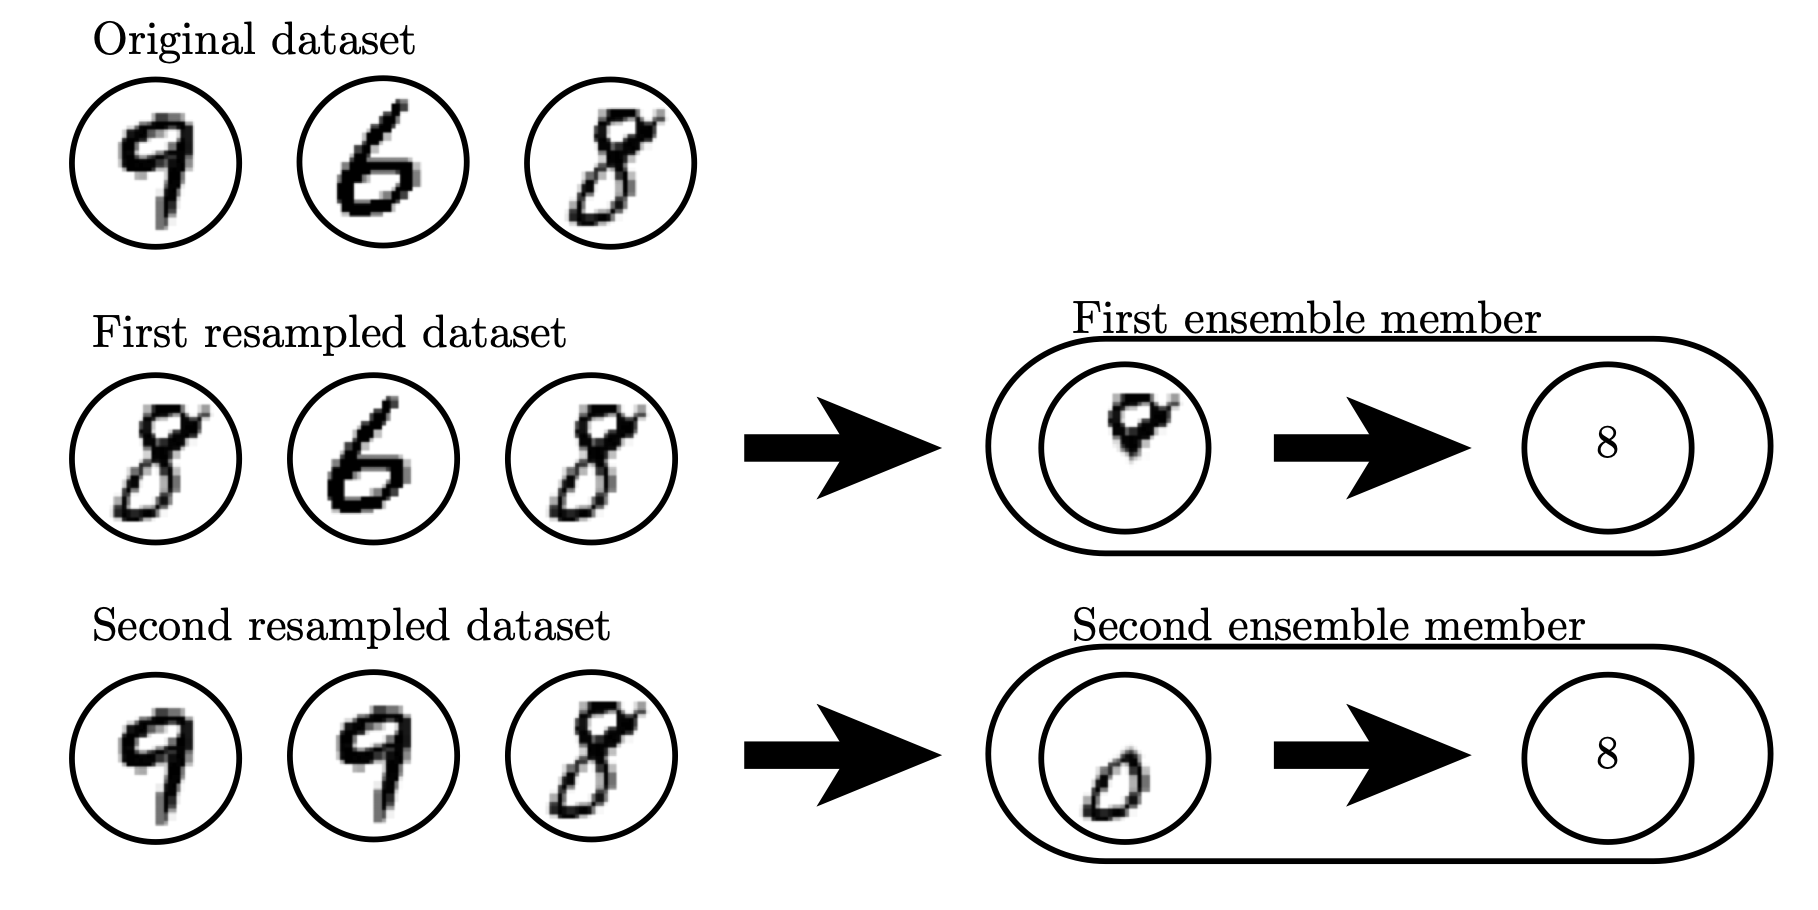
\includegraphics[width=0.75\textwidth]{../figures/week_1/bagging_cartoon.png}
    \end{center}
    \tiny{Figure from \cite{deeplearning}}
\end{frame}

\begin{frame}
\frametitle{Model averaging for neural networks}
    \begin{itemize}
        \item Neural networks profit from model averaging even when they are trained on the same data set.
        \item This is because with random initialization, minibatches (subsets of the training set), hyperparameters, non-determinism in the implementation a sufficient variety between the models can be achieved.
    \end{itemize}
\end{frame}


\begin{frame}
\frametitle{Model averaging in general}
    \begin{itemize}
        \item In general, it is considered that model averaging always improves the generalization error.
        \item In theory, with sufficient computer memory and time one can always improve the results by combining several methods.
        \item Therefore, when testing/benchmarking (new) methods it is considered "fair" to use only a single model.
        \item Machine learning contests are usually won by using model averaging.
        \item {\bf Boosting} is similar to ensembling, only the models (neural networks) are added {\bf incrementally} to the ensemble.
    \end{itemize}
\end{frame}

\fi % Ensambling


\begin{frame}
\frametitle{Important: introductory topics covered in video lecture}
These topics are covered in the extended slide stack and video lecture (links in Cavas) and are exam material:
\begin{itemize}
  \item Linear algebra
  \item Probability theory
  \item Maximum-likelihood estimation
  \item Supervised and unsupervised algorithms
  \item Ensambling
\end{itemize}
\end{frame}

\begin{frame}
\frametitle{Acknowledgements}

The slides for this lecture were prepared by Mitko Veta and Dragan Bo{\v s}nacki.

Some of the slides are based on the accompanying lectures of \cite{deeplearning}.

\end{frame}


\begin{frame}
\frametitle{References}
\printbibliography
\end{frame}

\end{document}
